% !TeX spellcheck = de-DE
% !TeX encoding = utf8
% !TeX program = lualatex
% !TeX TXS-program:compile = txs:///lualatex/[--shell-escape]
% !BIB program = biber
% -*- coding:utf-8 mod:LaTeX -*-

% vv  scroll down to line 200 for content  vv


\let\ifdeutsch\iftrue
\let\ifenglisch\iffalse
% EN: This file is loaded before the \documentclass command in the main document

% EN: The following package allows \\ at the title page
%     For more information see https://github.com/latextemplates/scientific-thesis-cover/issues/4
\RequirePackage{kvoptions-patch}

\ifenglisch
  \PassOptionsToClass{numbers=noenddot}{scrbook}
\else
  %()Aus scrguide.pdf - der Dokumentation von KOMA-Script)
  %Nach DUDEN steht in Gliederungen, in denen ausschließlich arabische Ziffern für die Nummerierung
  %verwendet werden, am Ende der Gliederungsnummern kein abschließender Punkt
  %(siehe [DUD96, R3]). Wird hingegen innerhalb der Gliederung auch mit römischen Zahlen
  %oder Groß- oder Kleinbuchstaben gearbeitet, so steht am Ende aller Gliederungsnummern ein
  %abschließender Punkt (siehe [DUD96, R4])
  \PassOptionsToClass{numbers=autoendperiod}{scrbook}
\fi

% Warns about outdated packages and missing caption declarations
% See https://www.ctan.org/pkg/nag
\RequirePackage[l2tabu, orthodox]{nag}

%DE: Neue deutsche Trennmuster
%    Siehe http://www.ctan.org/pkg/dehyph-exptl und http://projekte.dante.de/Trennmuster/WebHome
%    Nur für pdflatex, nicht für lualatex
\RequirePackage{ifluatex}
\ifluatex
  % do not load anything
\else
  \ifdeutsch
    \RequirePackage[ngerman=ngerman-x-latest]{hyphsubst}
  \fi
\fi

\documentclass[
  fontsize=12pt, % Vorgabe von Herrn Müller
  a4paper,  % Standard format - only KOMAScript uses paper=a4 - https://tex.stackexchange.com/a/61044/9075
  oneside,  % oneside für einseitigen Druck, twoside für buchartigen druck
  bibliography=totoc,
                 %idxtotoc,   %Index ins Inhaltsverzeichnis
  %               liststotoc, %List of X ins Inhaltsverzeichnis, mit liststotocnumbered werden die Abbildungsverzeichnisse nummeriert
  headsepline,
  cleardoublepage=empty,
  parskip=half,
  %               draft    % um zu sehen, wo noch nachgebessert werden muss - wichtig, da Bindungskorrektur mit drin
  draft=false
]{scrbook}
% !TeX encoding = utf8
% -*- coding:utf-8 mod:LaTeX -*-

% EN: This file includes basic packages and sets options. The order of package
%     loading is important
% DE: In dieser Datei werden zuerst die benoetigten Pakete eingebunden und
%     danach diverse Optionen gesetzt. Achtung Reihenfolge ist entscheidend!


%%%
% EN: Styleguide:
% - English comments are prefixed with "EN", German comments are prefixed with "DE"
% - Prefixed headings define the language for the subsequent paragraphs
% - It is tried to organize packages in blocks. One block starts with %%%, then
%   % <heading>, then the options and more text. % followed by %%% end a block.
%
% DE: Styleguide:
%
% Ein sehr kleiner Styleguide. Packages werden in Blöcken organisiert.
% Ein Block beginnt mit drei % in einer Zeile, dann % <Blocküberschrift>, dann
% eine Liste der möglichen Optionen und deren Einstellungen, Gründe und Kommentare
% eine % Zeile in der sonst nichts steht und dann wieder %%% in einer Zeile.
%
% Zwischen zwei Blöcken sind 2 Leerzeilen!
% Zu jedem Paket werden soviele Optionen wie möglich/nötig angegeben
%
%%%


%%%
% EN: Enable copy and paste of text from the PDF
%     Only required for pdflatex. It "just works" in the case of lualatex.
%     mmap enables mathematical symbols, but does not work with the newtx font set
%     See: https://tex.stackexchange.com/a/64457/9075
%     Other solutions outlined at http://goemonx.blogspot.de/2012/01/pdflatex-ligaturen-und-copynpaste.html and http://tex.stackexchange.com/questions/4397/make-ligatures-in-linux-libertine-copyable-and-searchable
%     Trouble shooting outlined at https://tex.stackexchange.com/a/100618/9075
\ifluatex
\else
  \usepackage{cmap}
\fi
%%%


%%%
% EN: File encoding
% DE: Codierung
%     Wir sind im 21 Jahrhundert, utf-8 löst so viele Probleme.
%
% Mit UTF-8 funktionieren folgende Pakete nicht mehr. Bitte beachten!
%   * fancyvrb mit §
%   * easylist -> http://www.ctan.org/tex-archive/macros/latex/contrib/easylist/
\ifluatex
  % EN: See https://tex.stackexchange.com/a/158517/9075
  %     Not required, because of usage of fontspec package
  %\usepackage[utf8]{luainputenc}
\else
  \usepackage[utf8]{inputenc}
\fi
%
%%%

%%%
% DE: Parallelbetrieb tex4ht und pdflatex
\makeatletter
\@ifpackageloaded{tex4ht}{
  \def\iftex4ht{\iftrue}
}{
  \def\iftex4ht{\iffalse}
}
\makeatother
%%%


%%%
% EN: Defintion of colors
% DE: Farbdefinitionen
\usepackage[hyperref,dvipsnames]{xcolor}
%

%%%
% EN: Required for custom acronyms/glossaries style.
%     Left aligned Columns in tables with fixed width.
%     See http://tex.stackexchange.com/questions/91566/syntax-similar-to-centering-for-right-and-left
\usepackage{ragged2e}
%%%

%%%
% EN: Abbreviations
% DE: Abkürzungsverzeichnis
%
% DE: Wichtig, ansonsten erscheint "No room for a new \write"
\usepackage{scrwfile}
% DE: siehe http://www.dickimaw-books.com/cgi-bin/faq.cgi?action=view&categorylabel=glossaries#glsnewwriteexceeded
\usepackage[acronym,indexonlyfirst,nomain]{glossaries}
%\usepackage[acronym,nomain]{glossaries}
\ifdeutsch
  \renewcommand*{\acronymname}{Abkürzungsverzeichnis}
\else
  \renewcommand*{\acronymname}{List of Abbreviations}
\fi
\renewcommand*{\glsgroupskip}{}
%
% EN: Removed Glossarie as a table as a quick fix to get the template working again
%     See http://tex.stackexchange.com/questions/145579/how-to-print-acronyms-of-glossaries-into-a-table
%
\makenoidxglossaries
%%%


%%%
% EN: Support for language-specific hyphenation
% DE: Neue deutsche Rechtschreibung und Literatur statt "Literature"
%     Die folgende Einstellung ist der Nachfolger von ngerman.sty
\ifdeutsch
  % DE: letzte Sprache ist default, Einbindung von "american" ermöglicht \begin{otherlanguage}{amercian}...\end{otherlanguage} oder \foreignlanguage{american}{Text in American}
  %     Siehe auch http://tex.stackexchange.com/a/50638/9075
  \usepackage[american,ngerman]{babel}
  % Ein "abstract" ist eine "Kurzfassung", keine "Zusammenfassung"
  \addto\captionsngerman{%
    \renewcommand\abstractname{Kurzfassung}%
  }
  \ifluatex
    % EN: conditionally disable ligatures. See https://github.com/latextemplates/scientific-thesis-template/issues/54
    %     for a discussion
    \usepackage[ngerman]{selnolig}
  \fi
\else
  % EN: Set English as language and allow to write hyphenated"=words
  %     `american`, `english` and `USenglish` are synonyms for babel package (according to https://tex.stackexchange.com/questions/12775/babel-english-american-usenglish).
  %      "english" has to go last to set it as default language
  \usepackage[ngerman,english]{babel}
  % EN: Hint by http://tex.stackexchange.com/a/321066/9075 -> enable "= as dashes
  \addto\extrasenglish{\languageshorthands{ngerman}\useshorthands{"}}
  \ifluatex
    % EN: conditionally disable ligatures. See https://github.com/latextemplates/scientific-thesis-template/issues/54
    %     for a discussion
    \usepackage[english]{selnolig}
  \fi
\fi
%
%%%


%%%
% EN: For easy quotations: \enquote{text}
%     This package is very smart when nesting is applied, otherwise textcmds (see below) provides a shorter command
% DE:  Anführungszeichen
%      Zitate in \enquote{...} setzen, dann werden automatisch die richtigen Anführungszeichen verwendet.
\usepackage{csquotes}
%%%


%%%
% EN: For even easier quotations: \qq{text}.
%     Is not smart in the case of nesting, but good enough for the most cases
\usepackage{textcmds}
\ifdeutsch
  % EN: German quotes are different. So do not use the English quotes, but the ones provided by the csquotes package.
  \renewcommand{\qq}[1]{\enquote{\emph{#1}}}
\fi
%%%


%%%
% EN: extended enumarations
% DE: erweitertes Enumerate
\usepackage{paralist}
%
%%%


%%%
% DE: fancyheadings (nicht nur) fuer koma
\usepackage[automark]{scrlayer-scrpage}
%
%%%


%%%
% EN: Mathematics
% DE: Mathematik
%
% DE: Viele Mathematik-Sachen. Siehe https://texdoc.net/pkg/amsmath
\usepackage{amsmath}
% EN: Options must be passed this way, otherwise it does not work with glossaries
\PassOptionsToPackage{fleqn,leqno}{amsmath}
% DE: fleqn (=Gleichungen linksbündig platzieren) funktioniert nicht direkt. Es muss noch ein Patch gemacht werden:
%\addtolength\mathindent{1em}%work-around ams-math problem with align and 9 -> 10. Does not work with glossaries, No visual changes.
% EN: Fixes bugs in AMS math
\usepackage{mathtools}
%
% EN: For theorems, replacement for amsthm
\usepackage[amsmath,hyperref]{ntheorem}
\theorempreskipamount 2ex plus1ex minus0.5ex
\theorempostskipamount 2ex plus1ex minus0.5ex
\theoremstyle{break}
\newtheorem{definition}{Definition}[section]
%
%%%


%%%
% DE: Intelligentes Leerzeichen um hinter Abkürzungen die richtigen Abstände zu erhalten, auch leere.
%     Siehe commands.tex \gq{}
\usepackage{xspace}
%DE: Macht \xspace und \enquote kompatibel
\makeatletter
\xspaceaddexceptions{\grqq \grq \csq@qclose@i \} }
\makeatother
%
%%%


%%%
% EN: Package for the appendix
% DE: Anhang
\usepackage{appendix}
%[toc,page,title,header]
%
%%%

%%%
% EN: Graphics
% DE: Grafikeinbindungen
%
% EN: The parameter "pdftex" is not required
\usepackage{graphicx}
\graphicspath{{\getgraphicspath}}
\newcommand{\getgraphicspath}{graphics/}
%
%%%


%%%
% EN: Enables inclusion of SVG graphics - 1:1 approach
%    This is NOT the approach of https://ctan.org/pkg/svg-inkscape,
%     which allows text in SVG to be typeset using LaTeX
%     We just include the SVG as is.
\usepackage{epstopdf}
\epstopdfDeclareGraphicsRule{.svg}{pdf}{.pdf}{%
  inkscape -z -D --file=#1 --export-pdf=\OutputFile
}
%
%%%


%%%
% EN: Enables inclusion of SVG graphics - text-rendered-with-LaTeX-approach
%     This is the approach of https://ctan.org/pkg/svg-inkscape,
\newcommand{\executeiffilenewer}[3]{%
  \IfFileExists{#2}
  {
    %\message{file #2 exists}
    \ifnum\pdfstrcmp{\pdffilemoddate{#1}}%
      {\pdffilemoddate{#2}}>0%
      {\immediate\write18{#3}}
    \else
      {%\message{file up to date #2}
      }
    \fi%
  }{
    %\message{file #2 doesn't exist}
    %\message{argument: #3}
    %\immediate\write18{echo "test" > xoutput.txt}
    \immediate\write18{#3}
  }
}
\newcommand{\includesvg}[1]{%
  \executeiffilenewer{#1.svg}{#1.pdf}%
  {
    inkscape -z -D --file=\getgraphicspath#1.svg %
    --export-pdf=\getgraphicspath#1.pdf --export-latex}%
  \input{\getgraphicspath#1.pdf_tex}%
}


%%%
% EN: Enable typesetting values with SI units.
\ifdeutsch
  \usepackage[mode=text,group-four-digits]{siunitx}
  \sisetup{locale=DE}
\else
  \usepackage[mode=text,group-four-digits,group-separator={,}]{siunitx}
  \sisetup{locale=US}
\fi
%%%

%%%
% EN: Extensions for tables
% DE: Tabellenerweiterungen
\usepackage{array} %increases tex's buffer size and enables ``>'' in tablespecs
\usepackage{longtable}
\usepackage{dcolumn} %Aligning numbers by decimal points in table columns
\ifdeutsch
  \newcolumntype{d}[1]{D{.}{,}{#1}}
\else
  \newcolumntype{d}[1]{D{.}{.}{#1}}
\fi
\setlength{\extrarowheight}{1pt}
%%%

%%%
% Eine Zelle, die sich über mehrere Zeilen erstreckt.
% Siehe Beispieltabelle in Kapitel 2
\usepackage{multirow}
%
%%%

%%%
%Fuer Tabellen mit Variablen Spaltenbreiten
%\usepackage{tabularx}
%\usepackage{tabulary}
%
%%%


%%%
% EN: Links behave as they should. Enables "\url{...}" for URL typesettings.
%     Allow URL breaks also at a hyphen, even though it might be confusing: Is the "-" part of the address or just a hyphen?
%     See https://tex.stackexchange.com/a/3034/9075.
% DE: Links verhalten sich so, wie sie sollen
%     Zeilenumbrüche bei URLs auch bei Bindestrichen erlauben, auch wenn es verwirrend sein könnte: Gehört der Bindestrich zur URL oder ist es ein Trennstrich?
%     Siehe https://tex.stackexchange.com/a/3034/9075.
\usepackage[hyphens]{url}
%
%  EN: When activated, use text font as url font, not the monospaced one.
%      For all options see https://tex.stackexchange.com/a/261435/9075.
% \urlstyle{same}
%
% EN: Hint by http://tex.stackexchange.com/a/10419/9075.
\makeatletter
\g@addto@macro{\UrlBreaks}{\UrlOrds}
\makeatother
%
%%%


%%%
% Index über Begriffe, Abkürzungen
%\usepackage{makeidx} makeidx ist out -> http://xindy.sf.net verwenden
%
%%%

%%%
%lustiger Hack fuer das Abkuerzungsverzeichnis
%nach latex durchlauf folgendes ausfuehren
%makeindex ausarbeitung.nlo -s nomencl.ist -o ausarbeitung.nls
%danach nochmal latex
%\usepackage{nomencl}
%    \let\abk\nomenclature %Deutsche Ueberschrift setzen
%          \renewcommand{\nomname}{List of Abbreviations}
%        %Punkte zw. Abkuerzung und Erklaerung
%          \setlength{\nomlabelwidth}{.2\hsize}
%          \renewcommand{\nomlabel}[1]{#1 \dotfill}
%        %Zeilenabstaende verkleinern
%          \setlength{\nomitemsep}{-\parsep}
%    \makenomenclature
%
%%%

%%%
% EN: Logic for TeX - enables if-then-else in commands
% DE: Logik für TeX
%     FÜr if-then-else @ commands.tex
\usepackage{ifthen}
%
%%%


%%%
% EN: Code Listings
% DE: Listings
\usepackage{listings}
\lstset{language=XML,
  showstringspaces=false,
  extendedchars=true,
  basicstyle=\footnotesize\ttfamily,
  commentstyle=\slshape,
  % DE: Original: \rmfamily, damit werden die Strings im Quellcode hervorgehoben. Zusaetzlich evtl.: \scshape oder \rmfamily durch \ttfamily ersetzen. Dann sieht's aus, wie bei fancyvrb
  stringstyle=\ttfamily,
  breaklines=true,
  breakatwhitespace=true,
  % EN: alternative: fixed
  columns=flexible,
  numbers=left,
  numberstyle=\tiny,
  basewidth=.5em,
  xleftmargin=.5cm,
  % aboveskip=0mm, %DE: deaktivieren, falls man lstlistings direkt als floating object benutzt (\begin{lstlisting}[float,...])
  % belowskip=0mm, %DE: deaktivieren, falls man lstlistings direkt als floating object benutzt (\begin{lstlisting}[float,...])
  captionpos=b
}

\ifluatex
\else
  % EN: Enable UTF-8 support - see https://tex.stackexchange.com/q/419327/9075
  \usepackage{listingsutf8}
  \lstset{inputencoding=utf8/latin1}
\fi

\ifdeutsch
  \renewcommand{\lstlistlistingname}{Verzeichnis der Listings}
\fi
%
%%%


%%%
% EN: Alternative to listings could be fancyvrb. Can be used together.
% DE: Alternative zu Listings ist fancyvrb. Kann auch beides gleichzeitig benutzt werden.
\usepackage{fancyvrb}
%
%EN: Font size for the normal text
%DE: Groesse fuer den Fliesstext. Falls deaktiviert: \normalsize
%\fvset{fontsize=\small}
%
%DE: Somit kann im Text ganz einfach §verbatim§ text gesetzt werden.
%    Disabled, because UTF-8 does not work any more and lualatex causes issues
%\DefineShortVerb{\§}
%
%EN: Shrink font size of listings
\RecustomVerbatimEnvironment{Verbatim}{Verbatim}{fontsize=\footnotesize}
\RecustomVerbatimCommand{\VerbatimInput}{VerbatimInput}{fontsize=\footnotesize}
%
%EN: Hack for fancyvrb based on http://newsgroups.derkeiler.com/Archive/Comp/comp.text.tex/2008-12/msg00075.html
%EN: Change of the solution: \Vref somehow collidated with cleveref/varioref as the output of \Vref{} was "Abschnitt 4.3 auf Seite 85"; therefore changed to \myVref -- so completely removed
\newcommand{\Vlabel}[1]{\label[line]{#1}\hypertarget{#1}{}}
\newcommand{\lref}[1]{\hyperlink{#1}{\FancyVerbLineautorefname~\ref*{#1}}}
%
%%%


%%%
% EN: Tunings of captions for floats, listings, ...
% DE: Bildunterschriften bei floats genauso formatieren wie bei Listings
%     Anpassung wird unten bei den newfloat-Deklarationen vorgenommen
%     https://www.ctan.org/pkg/caption2 is superseeded by this package.
\usepackage{caption}
%
%%%


%%%
% EN: Provides rotating figures, where the PDF page is also turned
% DE: Ermoeglicht es, Abbildungen um 90 Grad zu drehen
%     Alternatives Paket: rotating Allerdings wird hier nur das Bild gedreht, während bei lscape auch die PDF-Seite gedreht wird.
%     Das Paket lscape dreht die Seite auch nicht
\usepackage{pdflscape}
%
%%%


%%%
%EN: Required for proper environments of fancyvrb and lstlistings
%    There is also the newfloat pacakge (recommended by minted), but we currently have no expericene with that
%DE: Wird für fancyvrb und für lstlistings verwendet
\usepackage{float}
%
% EN: Alternative to float package
%\usepackage{floatrow}
%DE: zustäzlich für den Paramter [H] = Floats WIRKLICH da wo sie deklariert wurden paltzieren - ganz ohne Kompromisse
%    floatrow ist der Nachfolger von float
%    Allerdings macht floatrow in manchen Konstellationen Probleme. Deshalb ist das Paket deaktiviert.
%
% EN: See http://www.tex.ac.uk/cgi-bin/texfaq2html?label=floats
% DE: floats IMMER nach einer Referenzierung platzieren
%\usepackage{flafter}
%%%


%%%
% EN: For nested figures
% DE: Fuer Abbildungen innerhalb von Abbildungen
%     Ersetzt die Pakete subfigure und subfig - siehe https://tex.stackexchange.com/a/13778/9075
\usepackage[hypcap=true]{subcaption}
%
%%%


%%%
% EN: Extended support for footnotes
% DE: Fußnoten
%
%\usepackage{dblfnote}  %Zweispaltige Fußnoten
%
% Keine hochgestellten Ziffern in der Fußnote (KOMA-Script-spezifisch):
%\deffootnote[1.5em]{0pt}{1em}{\makebox[1.5em][l]{\bfseries\thefootnotemark}}
%
% Abstand zwischen Fußnoten vergrößern:
%\setlength{\footnotesep}{.85\baselineskip}
%
% EN: Following command disables the separting line of the footnote
% DE: Folgendes Kommando deaktiviert die Trennlinie zur Fußnote
%\renewcommand{\footnoterule}{}
%
\addtolength{\skip\footins}{\baselineskip} % Abstand Text <-> Fußnote
%
% Fußnoten immer ganz unten auf einer \raggedbottom-Seite
% fnpos kommt aus dem yafoot package
\usepackage{fnpos}
\makeFNbelow
\makeFNbottom
%
%%%


%%%
% EN: Variable page heights
% DE: Variable Seitenhöhen zulassen
\raggedbottom
%
%%%


%%%
% Falls die Seitenzahl bei einer Referenz auf eine Abbildung nur dann angegeben werden soll,
% falls sich die Abbildung nicht auf der selben Seite befindet...
\iftex4ht
  %tex4ht does not work well with vref, therefore we emulate vref behavior
  \newcommand{\vref}[1]{\ref{#1}}
\else
  \ifdeutsch
    \usepackage[ngerman]{varioref}
  \else
    \usepackage{varioref}
  \fi
\fi
%%%

%%%
% EN: More beautiful tables if one uses \toprule, \midrule, \bottomrule
% DE: Noch schoenere Tabellen als mit booktabs mit http://www.zvisionwelt.de/downloads.html
\usepackage{booktabs}
%
%\usepackage[section]{placeins}
%
%%%


%%%
% EN: Graphs and Automata
%
% TODO: Since version 3.0 (2013-10-01), it supports pdflatex via the auto-pst-pdf package
%       Requires -shell-escape
%\usepackage{gastex}
%%%


%%%
%
%\usepackage{multicol}
%\usepackage{setspace} % kollidiert mit diplomarbeit.sty
%%%


%%%
%biblatex statt bibtex
\usepackage[
  backend       = biber, %biber does not work with 64x versions alternative: bibtex8
  %minalphanames only works with biber backend
  %sortcites     = none, % sonst wird Nummerierung zerstört
  sorting       = none,
  bibstyle      = numeric, %alphabetic,
  citestyle     = numeric, %alphabetic,
  giveninits    = true,
  useprefix     = true, %"von, van, etc." will be printed, too. See below.
  minnames      = 1,
  minalphanames = 3,
  maxalphanames = 4,
  maxbibnames   = 3,
  maxcitenames  = 2,
  natbib        = true,
  eprint        = true,
  url           = true,
  doi           = true,
  isbn          = true,
  backref       = false]{biblatex}

% enable more breaks at URLs. See https://tex.stackexchange.com/a/134281.
\setcounter{biburllcpenalty}{7000}
\setcounter{biburlucpenalty}{8000}

\bibliography{bibliography}
%\addbibresource[datatype=bibtex]{bibliography.bib}

%Do not put "vd" in the label, but put it at "\citeauthor"
%Source: http://tex.stackexchange.com/a/30277/9075
\makeatletter
\AtBeginDocument{\toggletrue{blx@useprefix}}
\AtBeginBibliography{\togglefalse{blx@useprefix}}
\makeatother

%Thin spaces between initials
%http://tex.stackexchange.com/a/11083/9075
\renewrobustcmd*{\bibinitdelim}{\,}

%Keep first and last name together in the bibliography
%http://tex.stackexchange.com/a/196192/9075
\renewcommand*\bibnamedelimc{\addnbspace}
\renewcommand*\bibnamedelimd{\addnbspace}

%Replace last "and" by comma in bibliography
%See http://tex.stackexchange.com/a/41532/9075
\AtBeginBibliography{%
  \renewcommand*{\finalnamedelim}{\addcomma\space}%
}

\DefineBibliographyStrings{ngerman}{
  backrefpage  = {zitiert auf S\adddot},
  backrefpages = {zitiert auf S\adddot},
  andothers    = {et\ \addabbrvspace al\adddot},
  %Tipp von http://www.mrunix.de/forums/showthread.php?64665-biblatex-Kann-%DCberschrift-vom-Inhaltsverzeichnis-nicht-%E4ndern&p=293656&viewfull=1#post293656
  bibliography = {Literaturverzeichnis}
}

%enable hyperlinked author names when using \citeauthor
%source: http://tex.stackexchange.com/a/75916/9075
\DeclareCiteCommand{\citeauthor}
{\boolfalse{citetracker}%
  \boolfalse{pagetracker}%
  \usebibmacro{prenote}}
{\ifciteindex
  {\indexnames{labelname}}
  {}%
  \printtext[bibhyperref]{\printnames{labelname}}}
{\multicitedelim}
{\usebibmacro{postnote}}

%natbib compatibility
%\newcommand{\citep}[1]{\cite{#1}}
%\newcommand{\citet}[1]{\citeauthor{#1} \cite{#1}}
%Beginning of sentence - analogous to cleveref - important for names such as "zur Muehlen"
%\newcommand{\Citep}[1]{\cite{#1}}
%\newcommand{\Citet}[1]{\Citeauthor{#1} \cite{#1}}
%%%


%%%
% DE: Blindtext. Paket "blindtext" ist fortgeschritterner als "lipsum" und kann auch Mathematik im Text (http://texblog.org/2011/02/26/generating-dummy-textblindtext-with-latex-for-testing/)
%     kantlipsum (https://www.ctan.org/tex-archive/macros/latex/contrib/kantlipsum) ist auch ganz nett, aber eben auch keine Mathematik
%     Wird verwendet, um etwas Text zu erzeugen, um eine volle Seite wegen Layout zu sehen.
\usepackage[math]{blindtext}
%%%


%%%
% EN: Make LaTeX logos available by commands. E.g., \lualatex
\usepackage{dtk-logos}
%
%%%


%%%
% DE: Neue Pakete bitte VOR hyperref einbinden. Insbesondere bei Verwendung des
%     Pakets "index" wichtig, da sonst die Referenzierung nicht funktioniert.
%     Für die Indizierung selbst ist unter http://xindy.sourceforge.net
%     ein gutes Tool zu erhalten
%%%


%%%
%
% EN: Add new packages at this place
% DE: Hier also neue packages einbinden
%
%%%


%%%
% EN: Provides hyperlinks
%     Option "unicode" fixes umlauts in the PDF bookmarks - see https://tex.stackexchange.com/a/338770/9075
%
% DE: Erlaubt Hyperlinks im Dokument.
%     Alle Optionen nach \hypersetup verschoben, sonst crash
%     Siehe auch: "Praktisches LaTeX" - www.itp.uni-hannover.de/~kreutzm
\usepackage[unicode]{hyperref}
%

% EN: Define colors
% DE: Da es mit KOMA 3 und xcolor zu Problemen mit den global Options kommt MÜSSEN die Optionen so gesetzt werden.
%     Eigene Farbdefinitionen ohne die Namen des xcolor packages
\definecolor{darkblue}{rgb}{0,0,.5}
\definecolor{black}{rgb}{0,0,0}

% EN: Define color of links and more
\hypersetup{
  bookmarksnumbered=true,
  bookmarksopen=true,
  bookmarksopenlevel=1,
  breaklinks=true,
  colorlinks=true,
  pdfstartview=Fit,
  pdfpagelayout=SinglePage, % DE: Alterntaive: TwoPageRight -- zweiseitige Darstellung: ungerade Seiten rechts im PDF-Viewer - siehe auch http://tex.stackexchange.com/a/21109/9075
  %pdfencoding=utf8, % EN: This is probably the same as passing the option "unicode" at \usepackage{hyperref}
  filecolor=darkblue,
  urlcolor=darkblue,
  linkcolor=black,
  citecolor=black
}
%
%%%

%%%
% EN: Extensions for references inside the document (\cref{fig:sample}, ...)
% DE: cleveref für cref statt autoref, da cleveref auch bei Definitionen funktioniert
\ifdeutsch
  \usepackage[ngerman,capitalise,nameinlink,noabbrev]{cleveref}
\else
  \usepackage[capitalise,nameinlink,noabbrev]{cleveref}
\fi
%%%


%%%
% DE: Zur Darstellung von Algorithmen
%     Algorithm muss nach hyperref geladen werden
\usepackage[chapter]{algorithm}
\usepackage[]{algpseudocode}
%
%%%


%%%%%%%%%%%%%%%%%%%%%%%%%%%%%%%%%%%%%%%%%%%%%%%%%%%%%%%%%%%%%%%%%%%%%%%%%%%%%
%% EN: Fonts
%% DE: Schriften
%%
%% !!! If you change the font, be sure that words such as "workflow" can
%% !!! still be copied from the PDF. If this is not the case, you have
%% !!! to use glyphtounicode. See comment at cmap package
%%%%%%%%%%%%%%%%%%%%%%%%%%%%%%%%%%%%%%%%%%%%%%%%%%%%%%%%%%%%%%%%%%%%%%%%%%%%%

\automark[section]{chapter}
\setkomafont{pageheadfoot}{\normalfont\sffamily}
\setkomafont{pagenumber}{\normalfont\sffamily}
%
%\setheadsepline[.4pt]{.4pt} %funktioniert nicht: Alle Linien sind hier weg
%
%%%

%%%
% DE: Fuer deutsche Texte: Weniger Silbentrennung, mehr Abstand zwischen den Woertern
\ifdeutsch
  \setlength{\emergencystretch}{3em} % Silbentrennung reduzieren durch mehr frei Raum zwischen den Worten
\fi
%%%

% EN: Times Roman for all text
\ifluatex
  \usepackage{fontspec}
  \setmainfont{TeX Gyre Termes}
  \setsansfont[Scale=.9]{TeX Gyre Heros}
  \setmonofont[StylisticSet={1,3},Scale=.9]{inconsolata}
  \RequirePackage{newtxmath}
\else
  \RequirePackage{newtxtext}
  \RequirePackage{newtxmath}
  % EN: looks good with times, but no equivalent for lualatex found,
  %     therefore replaced with inconsolata
  %\RequirePackage[zerostyle=b,scaled=.9]{newtxtt}
  \RequirePackage[varl,scaled=.9]{inconsolata}
\fi

% EN: Fallback font - if the subsequent font packages do not define a font (e.g., monospaced)
%     This is the modern package for "Computer Modern".
% DE: Fallback-Schriftart
%\usepackage[%
%    rm={oldstyle=false,proportional=true},%
%    sf={oldstyle=false,proportional=true},%
%    tt={oldstyle=false,proportional=true,variable=true},%
%    qt=false%
%]{cfr-lm}

% EN: Headings are typset in Helvetica (which is similar to Arial)
% DE: Schriftart fuer die Ueberschriften - ueberschreibt lmodern
%\usepackage[scaled=.95]{helvet}

% DE: Für Schreibschrift würde tun, muss aber nicht
%\usepackage{mathrsfs} %  \mathscr{ABC}

% EN: Font for the main text
% DE: Schriftart fuer den Fliesstext - ueberschreibt lmodern
%     Linux Libertine, siehe http://www.linuxlibertine.org/
%     Packageparamter [osf] = Minuskel-Ziffern
%     rm = libertine im Brottext, Linux Biolinum NICHT als serifenlose Schrift, sondern helvet (von oben) beibehalten
%\usepackage[rm]{libertine}

% EN: Alternative Font: Palantino. It is recommeded by Prof. Ludewig for German texts
% DE: Alternative Schriftart: Palantino, Packageparamter [osf] = Minuskel-Ziffern
%     Bitte nur in deutschen Texten
%\usepackage{mathpazo} %ftp://ftp.dante.de/tex-archive/fonts/mathpazo/ - Tipp aus DE-TEX-FAQ 8.2.1

% DE: Schriftart fuer Programmcode - ueberschreibt lmodern
%     Falls auskommentiert, wird die Standardschriftart lmodern genommen
%     Fuer schreibmaschinenartige Schluesselwoerter in den Listings - geht bei alten Installationen nicht, da einige Fontshapes (<>=) fehlen
%\usepackage[scaled=.92]{luximono}
%\usepackage{courier}
% DE: BeraMono als Typewriter-Schrift, Tipp von http://tex.stackexchange.com/a/71346/9075
%\usepackage[scaled=0.83]{beramono}

% EN: backticks (`) are rendered as such in verbatim environments.
%     See following links for details:
%     - https://tex.stackexchange.com/a/341057/9075
%     - https://tex.stackexchange.com/a/47451/9075
%     - https://tex.stackexchange.com/a/166791/9075
\usepackage{upquote}

% DE: Symbole
%
%\usepackage[geometry]{ifsym} % \BigSquare
%\usepackage{mathabx}
%\usepackage{stmaryrd} %fuer \ovee, \owedge, \otimes
%\usepackage{marvosym} %fuer \Writinghand %patched to not redefine \Rightarrow
%\usepackage{mathrsfs} %mittels \mathscr{} schoenen geschwungenen Buchstaben erzeugen
%\usepackage{calrsfs} %\mathcal{} ein bisserl dickeren buchstaben erzeugen - sieht net so gut aus.
%durch mathpazo ist das schon definiert
\usepackage{amssymb}

% EN: For \texttrademark{}
\usepackage{textcomp}

% EN: name-clashes von marvosym und mathabx vermeiden:
\def\delsym#1{%
  %  \expandafter\let\expandafter\origsym\expandafter=\csname#1\endcsname
  %  \expandafter\let\csname orig#1\endcsname=\origsym
  \expandafter\let\csname#1\endcsname=\relax
}

%\usepackage{pifont}
%\usepackage{bbding}
%\delsym{Asterisk}
%\delsym{Sun}\delsym{Mercury}\delsym{Venus}\delsym{Earth}\delsym{Mars}
%\delsym{Jupiter}\delsym{Saturn}\delsym{Uranus}\delsym{Neptune}
%\delsym{Pluto}\delsym{Aries}\delsym{Taurus}\delsym{Gemini}
%\delsym{Rightarrow}
%\usepackage{mathabx} - Ueberschreibt leider zu viel - und die \le-Zeichen usw. sehen nicht gut aus!


%%%
% EN: Modern font encoding
%     Has to be loaded AFTER any font packages. See https://tex.stackexchange.com/a/2869/9075.
\ifluatex
\else
  \usepackage[T1]{fontenc}
\fi
%
%%%

%%
% EN: Character protrusion and font expansion. See http://www.ctan.org/tex-archive/macros/latex/contrib/microtype/
\usepackage[
  babel=true, % EN: Enable language-specific kerning. Take language-settings from the languge of the current document (see Section 6 of microtype.pdf)
  expansion=alltext,
  protrusion=alltext-nott, % EN: Ensure that at listings, there is no change at the margin of the listing
  final % EN: Always enable microtype, even if in draft mode. This helps finding bad boxes quickly.
        %     In the standard configuration, this template is always in the final mode, so this option only makes a difference if "pros" use the draft mode
]{microtype}
%
% EN: \texttt{test -- test} keeps the "--" as "--" (and does not convert it to an en dash)
\DisableLigatures{encoding = T1, family = tt* }
%
%DE: fuer microtype
%DE: tracking=true muss als Parameter des microtype-packages mitgegeben werden
%DE: Deaktiviert, da dies bei Algorithmen seltsam aussieht
%
%\DeclareMicrotypeSet*[tracking]{my}{ font = */*/*/sc/* }%
%\SetTracking{ encoding = *, shape = sc }{ 45 }
%DE: Hier wird festgelegt,
%    dass alle Passagen in Kapitälchen automatisch leicht
%    gesperrt werden.
%    Quelle: http://homepage.ruhr-uni-bochum.de/Georg.Verweyen/pakete.html
%    Deaktiviert, da sonst "BPEL", "BPMN" usw. wirklich komisch aussehen.
%    Macht wohl nur bei geisteswissenschaftlichen Arbeiten Sinn.
%%%

%%%
% CTAN: https://ctan.org/pkg/lccaps
% Doc: http://texdoc.net/pkg/lccaps
%
% Required for DE/EN \initialism
\usepackage{lccaps}
%%%

%%%
% Links auf Gleitumgebungen springen nicht zur Beschriftung,
% Doc: http://mirror.ctan.org/tex-archive/macros/latex/contrib/oberdiek/hypcap.pdf
% sondern zum Anfang der Gleitumgebung
\usepackage[all]{hypcap}
%%%


%%%
% Deckblattstyle
%
\ifdeutsch
  \PassOptionsToPackage{language=german}{scientific-thesis-cover}
\else
  \PassOptionsToPackage{language=english}{scientific-thesis-cover}
\fi


%%%
%Bugfixes packages
%\usepackage{fixltx2e} %Fuer neueste LaTeX-Installationen nicht mehr benoetigt - bereinigte einige Ungereimtheiten, die auf Grund von Rueckwaertskompatibilitaet beibahlten wurden.
%\usepackage{mparhack} %Fixt die Position von marginpars (die in DAs selten bis gar nicht gebraucht werden}
%\usepackage{ellipsis} %Fixt die Abstaende vor \ldots. Wird wohl auch nicht benoetigt.
%
%%%


%%%
% EN: Settings for captions of floats
% DE: Formatierung der Beschriftungen
%
\captionsetup{
  format=hang,
  labelfont=bf,
  justification=justified,
  %single line captions should be centered, multiline captions justified
  singlelinecheck=true
}
%
% EN: New float environments for listings and algorithms
%
% \floatstyle{ruled} % TODO: enabled or disabled causes no change - listings and algorithms are always ruled
%
\newfloat{Listing}{tbp}{code}[chapter]
\crefname{Listing}{Listing}{Listings}
%
\newfloat{Algorithmus}{tbp}{alg}[chapter]
\ifdeutsch
  \crefname{Algorithmus}{Algorithmus}{Algorithmus}
\else
  \crefname{Algorithmus}{Algorithm}{Algorithms}
  \floatname{Algorithmus}{Algorithm}
\fi
%%


%%
%amsmath
%\numberwithin{equation}{section}
%\renewcommand{\theequation}{\thesection.\Roman{equation}}
%%


%%%
%EN: Various chapter styles
% DE: unterschiedliche Chapter-Styles
%     u.a. Paket fncychap

% Andere Kapitelueberschriften
% falls einem der Standard von KOMA nicht gefaellt...
% Falls man zurück zu KOMA moechte, dann muss jede der vier folgenden Moeglichkeiten deaktiviert sein.

%\usepackage[Sonny]{fncychap}

%\usepackage[Bjarne]{fncychap}

%\usepackage[Lenny]{fncychap}

%DE: Zur Aktivierung eines der folgenden Möglichkeiten ein Paar von "\iffalse" und "\fi" auskommentieren

\iffalse
  \usepackage[Bjarne]{fncychap}
  \ChNameVar{\Large\sf} \ChNumVar{\Huge} \ChTitleVar{\Large\sf}
  \ChRuleWidth{0.5pt} \ChNameUpperCase
\fi

\iffalse
  \usepackage[Rejne]{fncychap}
  \ChNameVar{\centering\Huge\rm\bfseries}
  \ChNumVar{\Huge}
  \ChTitleVar{\centering\Huge\rm}
  \ChNameUpperCase
  \ChTitleUpperCase
  \ChRuleWidth{1pt}
\fi

\iffalse
  \usepackage{fncychap}
  \ChNameUpperCase
  \ChTitleUpperCase
  \ChNameVar{\raggedright\normalsize} %\rm
  \ChNumVar{\bfseries\Large}
  \ChTitleVar{\raggedright\Huge}
  \ChRuleWidth{1pt}
\fi

\iffalse
  \usepackage[Bjornstrup]{fncychap}
  \ChNumVar{\fontsize{76}{80}\selectfont\sffamily\bfseries}
  \ChTitleVar{\raggedright\Large\sffamily\bfseries}
\fi

% EN: Complete different chapter style - self made

% Innen drin kann man dann noch zwischen
%   * serifenloser Schriftart (eingestellt)
%   * serifenhafter Schriftart (wenn kein zusaetzliches Kommando aktiviert ist) und
%   * Kapitälchen wählen
\iffalse
  \makeatletter
  %\def\thickhrulefill{\leavevmode \leaders \hrule height 1ex \hfill \kern \z@}

  %Fuer Kapitel mit Kapitelnummer
  \def\@makechapterhead#1{%
    \vspace*{10\p@}%
    {\parindent \z@ \raggedright \reset@font
      %Default-Schrift: Serifenhaft (gut fuer englische Dokumente)
      %A) Fuer serifenlose Schrift:
      \fontfamily{phv}\selectfont
      %B) Fuer Kapitaelchen:
      %\fontseries{m}\fontshape{sc}\selectfont
      %C) Fuer ganz "normale" Schrift:
      %\normalfont
      %
      \Large \@chapapp{} \thechapter
      \par\nobreak\vspace*{10\p@}%
      \interlinepenalty\@M
      {\Huge\bfseries\baselineskip3ex
        %Fuer Kapitaelchen folgende Zeile aktivieren:
        %\fontseries{m}\fontshape{sc}\selectfont
        #1\par\nobreak}
      \vspace*{10\p@}%
      \makebox[\textwidth]{\hrulefill}%    \hrulefill alone does not work
      \par\nobreak
      \vskip 40\p@
    }}

  %Fuer Kapitel ohne Kapitelnummer (z.B. Inhaltsverzeichnis)
  \def\@makeschapterhead#1{%
    \vspace*{10\p@}%
    {\parindent \z@ \raggedright \reset@font
      \normalfont \vphantom{\@chapapp{} \thechapter}
      \par\nobreak\vspace*{10\p@}%
      \interlinepenalty\@M
      {\Huge \bfseries %
        %Default-Schrift: Serifenhaft (gut fuer englische Dokumente)
        %A) Fuer serifenlose Schrift folgende Zeile aktivieren:
        \fontfamily{phv}\selectfont
        %B) Fuer Kapitaelchen folgende Zeile aktivieren:
        %\fontseries{m}\fontshape{sc}\selectfont
        #1\par\nobreak}
      \vspace*{10\p@}%
      \makebox[\textwidth]{\hrulefill}%    \hrulefill does not work
      \par\nobreak
      \vskip 40\p@
    }}
  %
  \makeatother
\fi
%%%

%%%
%Minitoc-Einstellungen
%\dominitoc
%\renewcommand{\mtctitle}{Inhaltsverzeichnis dieses Kapitels}
%%%

%%%
% EN: Nicer paragraph line placement:
%     - Disable single lines at the start of a paragraph (Schusterjungen)
%     - Disable single lines at the end of a paragraph (Hurenkinder)
%     Normally, this is clubpenalty and widowpenalty, but using a package, it feels more non-hacky
\usepackage[all,defaultlines=3]{nowidow}
%
\displaywidowpenalty = 10000
%%%

%%%
% EN: Try to get rid of "overfull hbox" things and let text flow batter
%     See also
%       - http://groups.google.de/group/de.comp.text.tex/browse_thread/thread/f97da71d90442816/f5da290593fd647e?lnk=st&q=tolerance+emergencystretch&rnum=5&hl=de#f5da290593fd647e
%       - http://www.tex.ac.uk/cgi-bin/texfaq2html?label=overfull
\tolerance=2000
%
% EN: This could be increased to 20pt
\setlength{\emergencystretch}{3pt}
%
% EN: Suppress hbox warnings if less than 1pt
\setlength{\hfuzz}{1pt}
%
%%%


%%%
% EN: Fix names for algorithms in German
% DE: fuer algorithm.sty: - falls Deutsch und nicht Englisch.
\ifdeutsch
  \floatname{algorithm}{Algorithmus}
  \renewcommand{\listalgorithmname}{Verzeichnis der Algorithmen}
\fi
%
%%%


%%%
% EN: The euro sign
% DE: Das Euro Zeichen
%     Fuer Palatino (mathpazo.sty): richtiges Euro-Zeichen
%     Alternative: \usepackage{eurosym}
\newcommand{\EUR}{\ppleuro}
%
%%%


%%%
%
% Float-placements - http://dcwww.camd.dtu.dk/~schiotz/comp/LatexTips/LatexTips.html#figplacement
% and http://people.cs.uu.nl/piet/floats/node1.html
\renewcommand{\topfraction}{0.85}
\renewcommand{\bottomfraction}{0.95}
\renewcommand{\textfraction}{0.1}
\renewcommand{\floatpagefraction}{0.75}
%\setcounter{totalnumber}{5}
%
%%%

%%%
%
% Bei Gleichungen nur dann die Nummer zeigen, wenn die Gleichung auch referenziert wird
%
% Funktioniert mit MiKTeX Stand 2012-01-13 nicht. Deshalb ist dieser Schalter deaktiviert.
%
%\mathtoolsset{showonlyrefs}
%
%%%


%%%
%ensure that floats covering a whole page are placed at the top of the page
%see http://tex.stackexchange.com/a/28565/9075
\makeatletter
\setlength{\@fptop}{0pt}
\setlength{\@fpbot}{0pt plus 1fil}
\makeatother
%%%


%%%
% EN: Improves the border of the text
% DE: Optischer Randausgleich und Grauwertkorrektur
\usepackage{microtype}
%%%

%%%
% EN: Margins
% DE: Ränder
%     Viele Moeglichkeiten, die Raender im Dokument einzustellen.
%
%     Satzspiegel neu berechnen. Dokumentation dazu ist in "scrguide.pdf" von KOMA-Skript zu finden
%     Optionen werden bei \documentclass[] in ausarbeitung.tex mitgegeben.
% \typearea[current]{current} %neu berechnen, da neue Schrift eingebunden

%\usepackage{a4}
%\usepackage{a4wide}
%\areaset{170mm}{277mm} %a4:29,7hochx21mbreit

%Wer die Masse direkt eingeben moechte:
%Bei diesem Beispiel wird die Regel nicht beachtet, dass der innere Rand halb so gross wie der aussere Rand und der obere Rand halb so gross wie der untere Rand sein sollte
%\usepackage[inner=2.5cm, outer=2.5cm, includefoot, top=3cm, bottom=1.5cm]{geometry}

% EN: Package geometry to enlarge on page
%
%     Normally, geometry should not be used as the typearea package calculates the margins perfectly for printing
%     However, we want better screen-readable documents where the content does not "jump"
%     Thus, we fix the margins left and right to the same value
%
%     Source: http://www.howtotex.com/tips-tricks/change-margins-of-a-single-page/
%
\usepackage[
  left=3cm,right=3cm,top=2.5cm,bottom=2.5cm,
  headsep=18pt,
  footskip=30pt,
  includehead,
  includefoot
]{geometry}
%%%


%%%
% EN: Provides todo notes
% DE: schoene TODOs
\ifdeutsch
  \usepackage[colorinlistoftodos,ngerman]{todonotes}
\else
  \usepackage[colorinlistoftodos]{todonotes}
\fi
\setlength{\marginparwidth}{2,5cm}

\let\xtodo\todo
\renewcommand{\todo}[1]{\xtodo[inline,color=black!5]{#1}}
\newcommand{\utodo}[1]{\xtodo[inline,color=green!5]{#1}}
\newcommand{\itodo}[1]{\xtodo[inline]{#1}}
%
%%%


%%%
% EN: Enable footnotes in tables.
%     This package superseeds the 1997 package "footnote"
\usepackage{footnotehyper}
% TODO: The footnotehyper author recommends to enclose the respective area with \begin{savenotes} ... \end{savenotes}
\makesavenoteenv{tabular}
\makesavenoteenv{table}
% Reuse of footnotes, see http://tex.stackexchange.com/questions/10102/multiple-references-to-the-same-footnote-with-hyperref-support-is-there-a-bett
\crefformat{footnote}{#2\footnotemark[#1]#3}
%%%


%%%
% EN: pgfplots (optional if the ppackage is installed)
%     PGFPlots draws high-qual­ity func­tion plots in nor­mal or log­a­rith­mic scal­ing
\IfFileExists{pgfplots.sty}{
  \usepackage{pgfplots}
  % EN: highest version supported by overleaf as of 2018-03-16
  \pgfplotsset{compat=1.14}
}{}
%%%

%%%
% EN: pgfplotstable (optional if the ppackage is installed)
%     PGFPlots generates tables from csv files
\IfFileExists{pgfplotstable.sty}{
  \usepackage{pgfplotstable}
}{}
%%%

%%%
% EN: Package for creating graphics programmatically
\usepackage{tikz}
%%%

%%%
% EN: tikz-uml
%     Package for creating uml diagramms
\usepackage{tikz-uml}
%%%

%%%
% EN: Enable PlantUML listings in the environment "plantuml"
\IfFileExists{plantuml.sty}{
  \usepackage[output=latex]{plantuml}
}{}
%%

%%
% EN: Layout: bottoms of pages not aligned to each other
% DE: Der untere Rand darf "flattern"
\raggedbottom
%%


%%%
% Wie tief wird das Inhaltsverzeichnis aufgeschlüsselt
% 0 --\chapter
% 1 --\section % fuer kuerzeres Inhaltsverzeichnis verwenden - oder minitoc benutzen
% 2 --\subsection
% 3 --\subsubsection
% 4 --\paragraph
\setcounter{tocdepth}{1}
%
%%%


%%%
% DE: Angaben in die PDF-Infos uebernehmen
\makeatletter
\hypersetup{
  pdftitle={}, %Titel der Arbeit
  pdfauthor={Lukas Willburger}, %Author
  pdfkeywords={}, % CR-Klassifikation und ggf. weitere Stichworte
  pdfsubject={}
}
\makeatother
%%%

%%%
% EN: Higher compression of the output PDF
\pdfcompresslevel=9
%%%


%%%
% EN: Required for recent version of komascript, as some packges are not that compatible with KOMAScript as they should be
%     Has to be loaded at the *very* end, so we use "\AtEndPreamble" by etoolsbox
\usepackage{etoolbox}
\AtEndPreamble{\usepackage{scrhack}}
%%%

%%%
% EN: Provide tables over multiple pages
\usepackage{longtable}
%%%

%%%
% EN: Show LaTeX commands and their results in the document
\usepackage{latexdemo}
%%%

%\setcounter{tocdepth}{4}
%%%
% EN: Syntax highligthing using pygments package
\usepackage[chapter]{minted}
\usepackage{titlesec}

\usepackage{wrapfig}
\usepackage{lipsum}

%\usepackage[ngerman]{babel}% deutsche Trennregeln
%\usepackage[T1]{fontenc}% wichtig für Trennung von Wörtern mit Umlauten
%\usepackage{microtype}% verbesserter Randausgleich

\usepackage[a4paper,%
  head=15mm,
  headsep=5mm,
  bottom=25mm,
  left=35mm,
  right=15mm, 
  footskip=10mm]{geometry}

\addtokomafont{chapter}{\LARGE} % kleinere Schrift für Kapitelüberschriften

\RedeclareSectionCommand[beforeskip=2sp, afterskip=1sp]{chapter}
\RedeclareSectionCommands[beforeskip=1sp, afterskip=1sp]{section,subsection,subsubsection}
\RedeclareSectionCommands[beforeskip=1sp, afterskip=1sp]{paragraph,subparagraph}

% EN: line numbers within page margins
% DE: Zeilennummern innerhalb vom Rand
\setminted{numbersep=5pt, xleftmargin=12pt, fontsize=\huge, baselinestretch=1}
%%%

%http://www.jevon.org/wiki/Eclipse_Pygments_Style
%\usemintedstyle{eclipse}
%
%\usemintedstyle{autumn}
%\usemintedstyle{rrt}
%\usemintedstyle{borland}
%\usemintedstyle{friendlygrayscale}
\usemintedstyle{friendly}

%EN: compatibility of packages minted and listings with respect to the numbering of "List." caption
%    source: https://tex.stackexchange.com/a/269510/9075
\AtBeginEnvironment{listing}{\setcounter{listing}{\value{lstlisting}}}
\AtEndEnvironment{listing}{\stepcounter{lstlisting}}
%EN: We use the Listing environment to have the nice bar. So, we also have to patch the "Listing" environment for consistent counters
\AtBeginEnvironment{Listing}{\setcounter{listing}{\value{lstlisting}}}
\AtEndEnvironment{Listing}{\stepcounter{lstlisting}}

% Abkürzungsverzeichnis



\makeindex
\usepackage{setspace} % Vorgabe von Herrn Müller
\onehalfspacing
\begin{document}

%----------------------------------------------------------------------------------------
%	TITELSEITE
%----------------------------------------------------------------------------------------
% Im Anhang Credit (CC BY 4.0!) für https://www.overleaf.com/latex/templates/uppsala-university-template/jvjprsfnzgbj#.WzX_c9IzaUk
\begin{titlepage}

\newcommand{\HRule}{\rule{\linewidth}{0.5mm}} % Defines a new command for the horizontal lines, change thickness here

\center % Center everything on the page
 
%----------------------------------------------------------------------------------------
%	HEADING SECTIONS
%----------------------------------------------------------------------------------------

\textsc{\LARGE Studienarbeit}\\[1.5cm] % Name of your university/college

\includegraphics[scale=.15]{logos/Logo_Hochschule_Kempten.png}\\[1cm] % Include a department/university logo - this will require the graphicx package
\textsc{\Large Seminar Blockchain }\\[0.5cm] % Major heading such as course name
%\vspace{2cm}
{\Large Sommersemester 2019} % Date, change the \today to a set date if you want to be precise
%\textsc{\large Course code}\\[0.5cm] % Minor heading such as course title

%----------------------------------------------------------------------------------------
%	TITLE SECTION
%----------------------------------------------------------------------------------------
\vspace{2.5cm}
{ \huge \bfseries Anwendungen von Smart Contracts }% Title of your document
\vspace{2.5cm}
 
%----------------------------------------------------------------------------------------
%	AUTHOR SECTION
%----------------------------------------------------------------------------------------

\begin{minipage}{0.4\textwidth}

\emph{Autor:}\\
Lukas \textsc{Willburger}\\ % Your name
Matrikelnr. 322445 \\
Master Informatik, 1. Semester \\ \newline 


\emph{Seminarleitung: }\\
Prof. Nikolaus \textsc{Steger} \\ \newline  \newline

\end{minipage}\\[1cm]

% If you don't want a supervisor, uncomment the two lines below and remove the section above
%\Large \emph{Author:}\\
%John \textsc{Smith}\\[3cm] % Your name

%----------------------------------------------------------------------------------------
%	DATE SECTION
%----------------------------------------------------------------------------------------



\vfill % Fill the rest of the page with whitespace

\end{titlepage}

\pagenumbering{gobble}
%tex4ht-Konvertierung verschönern
\iftex4ht
  % tell tex4ht to create picures also for formulas starting with '$'
  % WARNING: a tex4ht run now takes forever!
  \Configure{$}{\PicMath}{\EndPicMath}{}
  %$ % <- syntax highlighting fix for emacs
  \Css{body {text-align:justify;}}

  %conversion of .pdf to .png
  \Configure{graphics*}
  {pdf}
  {\Needs{"convert \csname Gin@base\endcsname.pdf
      \csname Gin@base\endcsname.png"}%
    \Picture[pict]{\csname Gin@base\endcsname.png}%
  }
\fi

%\VerbatimFootnotes %verbatim text in Fußnoten erlauben. Geht normalerweise nicht.
% DE: wird fuer Tabellen benötigt (z.B. >{centering\RBS}p{2.5cm} erzeugt einen zentrierten 2,5cm breiten Absatz in einer Tabelle
\newcommand{\RBS}{\let\\=\tabularnewline}

% EN: To avoid issues with Springer's \mathplus
%     See also http://tex.stackexchange.com/q/212644/9075
\providecommand\mathplus{+}

% DE: typoraphisch richtige Abkürzungen
\newcommand{\zB}{z.\,B.\xspace}
\newcommand{\bzw}{bzw.\xspace}
\newcommand{\usw}{usw.\xspace}
\renewcommand{\dh}{d.\,h.\xspace}

% EN: from hmks makros.tex - \indexify
\newcommand{\toindex}[1]{\index{#1}#1}

% DE: Tipp aus "The Comprehensive LaTeX Symbol List"
\newcommand{\dotcup}{\ensuremath{\,\mathaccent\cdot\cup\,}}

% DE: Anstatt $|x|$ $\abs{x}$ verwenden.
%     Die Betragsstriche skalieren automatisch, falls "x" etwas größer sein sollte...
\newcommand{\abs}[1]{\left\lvert#1\right\rvert}

% DE: für Zitate
\newcommand{\citeS}[2]{\cite[S.~#1]{#2}}
\newcommand{\citeSf}[2]{\cite[S.~#1\,f.]{#2}}
\newcommand{\citeSff}[2]{\cite[S.~#1\,ff.]{#2}}
\newcommand{\vgl}{vgl.\ }
\newcommand{\Vgl}{Vgl.\ }

% EN: For the algorithmic package
\newcommand{\commentchar}{\ensuremath{/\mkern-4mu/}}
\algrenewcommand{\algorithmiccomment}[1]{\hfill $\commentchar$ #1}

% DE: Seitengrößen - Gegen Schusterjungen und Hurenkinder...
\newcommand{\largepage}{\enlargethispage{\baselineskip}}
\newcommand{\shortpage}{\enlargethispage{-\baselineskip}}

\newcommand{\initialism}[1]{%
  \ifdeutsch%
    \textsc{#1}\xspace%
  \else%
    \textlcc{#1}\xspace%
  \fi%
}
\newcommand{\OMG}{\initialism{OMG}}
\newcommand{\BPEL}{\initialism{BPEL}}
\newcommand{\BPMN}{\initialism{BPMN}}
\newcommand{\UML}{\initialism{UML}}



%Eigener Seitenstil fuer die Kurzfassung und das Inhaltsverzeichnis
%\deftripstyle{preamble}{}{}{}{}{}{\pagemark}
%Doku zu deftripstyle: scrguide.pdf
%\pagestyle{preamble}
%\renewcommand*{\chapterpagestyle}{preamble}



%Kurzfassung / abstract
%auch im Stil vom Inhaltsverzeichnis
%\ifdeutsch
%  \section*{Kurzfassung}
%\else
%  \section*{Abstract}
%\fi
%
%... Short summary of the thesis ...
%
%\cleardoublepage


% BEGIN: Verzeichnisse

\iftex4ht
\else
  \microtypesetup{protrusion=false}
\fi

%%%
% Literaturverzeichnis ins TOC mit aufnehmen, aber nur wenn nichts anderes mehr hilft!
% \addcontentsline{toc}{chapter}{Literaturverzeichnis}
%
% oder zB
%\addcontentsline{toc}{section}{Abkürzungsverzeichnis}
%
%%%

%Produce table of contents
%
%In case you have trouble with headings reaching into the page numbers, enable the following three lines.
%Hint by http://golatex.de/inhaltsverzeichnis-schreibt-ueber-rand-t3106.html
%
%\makeatletter
%\renewcommand{\@pnumwidth}{2em}
%\makeatother
%

\tableofcontents

% Bei einem ungünstigen Seitenumbruch im Inhaltsverzeichnis, kann dieser mit
% \addtocontents{toc}{\protect\newpage}
% an der passenden Stelle im Fließtext erzwungen werden.

%Auflistung der Codezeilen
%\listoffigures

%Auflistung der Tabellen
%\listoftables

%Wird nur bei Verwendung von der lstlisting-Umgebung mit dem "caption"-Parameter benoetigt
%\lstlistoflistings
%ansonsten:
%\ifdeutsch
%  \listof{Listing}{Verzeichnis der Listings}
%\else
%  \listof{Listing}{List of Listings}
%\fi

%mittels \newfloat wurde die Algorithmus-Gleitumgebung definiert.
%Mit folgendem Befehl werden alle floats dieses Typs ausgegeben
%\ifdeutsch
%\listof{Algorithmus}{Verzeichnis der Algorithmen}
%\else
  %\listof{Algorithmus}{List of Algorithms}
%\fi
%\listofalgorithms %Ist nur für Algorithmen, die mittels \begin{algorithm} umschlossen werden, nötig
% Abkürzungsverzeichnis

%\printnoidxglossaries
\thispagestyle{empty}
\iftex4ht
\else
  %Optischen Randausgleich und Grauwertkorrektur wieder aktivieren
  \microtypesetup{protrusion=true}
\fi

% END: Verzeichnisse


% Headline and footline
\renewcommand*{\chapterpagestyle}{scrplain}
\pagestyle{scrheadings}
\pagestyle{scrheadings}
\ihead[]{}
\chead[]{}
\ohead[]{\headmark}
\cfoot[]{}
\ofoot[\usekomafont{pagenumber}\thepage]{\usekomafont{pagenumber}\thepage}
\ifoot[]{}



%-----------------------------------------------------------------------------
%
% Main content starts here
%
%-----------------------------------------------------------------------------
\pagenumbering{arabic}
\clearpage
\setcounter{page}{1}
% Hier stehen gesammelt alle Inhaltskapitel drin
\spacing{1.3}
% Hier können die einzelnen Kapitel inkludiert werden. Sie müssen in den 
% entsprechenden .TEX-Dateien vorliegen. Die Dateinamen können natürlich 
% angepasst werden.
\chapter{Einleitung}
\label{chap:Einleitung}
Die Blockchain-Technologie hat sich in den letzten Jahren zu einem regelrechten Hype-Thema entwickelt. So ist es nicht verwunderlich, dass alleine in Berlin im Jahr 2018 bereits 64 Blockchain-Startups niedergelassen waren \cite{AnzahlStartups2018}. Kryptowährungen, wie beispielsweise Bitcoin oder Ethereum, sind meist die erste Assoziation, die der Begriff Blockchain hervorruft. Über deren Sinn und Daseinsberechtigung im Geldmarkt wird seit Beginn angeregt diskutiert. So sagte der amerikanische Großinvestor Warren Buffet 2014 in einem Interview mit dem US-amerikanischen Sender CNBC über Bitcoin: \qq{Stay away from it. It’s a mirage, basically} \cite{Buffett2014}.

Es muss auch angemerkt werden, dass die Blockchain längst nicht mehr ausschließlich für Kryptowährungen bereitsteht. Mit der kontinuierlichen Weiterentwicklung avancierten vor allem die sogenannten \textit{Smart Contracts} zu einem wichtigen Bestandteil der Plattformen \cite[vgl.][S.~8]{Schuette2017}. Diese sind vor allem im Geschäftsleben von großem Interesse.

Werden in einem realen Umfeld Absprachen getroffen, stehen für beide Vertragsparteien Forderungen und zu erbringende Leistungen im Vordergrund. In bestimmten Fällen kann nicht auf deren Einhaltung vertraut werden, wodurch sich der Einsatz von Smart Contracts anbietet. Dadurch wird einerseits durch die technologische Architektur der Blockchain Manipulationssicherheit garantiert, als auch die Nachvollziehbarkeit aller geschäftlichen Transaktionen gewährleistet.

Einige Szenarien sollen in dieser Arbeit beispielhaft anhand von Use Cases der vorgestellten Unternehmen dargelegt werden. 
\chapter{Überblick}
\label{chap:Ueberblick}

\textit{Anmerkung: Da die Grundlagen von Ethereum Smart Contracts Bestandteil eines dieser Arbeit vorausgegangenen Seminarvortrags sind, wird auf deren Definition und weitere Einzelheiten an dieser Stelle nicht weiter eingegangen. Ein Grundlagenwissen zur Thematik gilt als vorausgesetzt.}

Sucht man mit den gängigen Suchmaschinen nach Smart Contract Anwendungen, so fällt auf, dass viele der gelisteten Suchergebnisse lediglich mögliche Szenarien beschreiben, ohne konkrete Anwendungsfälle beziehungsweise anwendende Unternehmen zu nennen. Bei einem genaueren Blick auf die Webseiten bestätigt sich die anfängliche Vermutung, dass viele Personen möglichst viel vom Hype um Blockchain und Bitcoin profitieren wollen. \\
Dennoch lassen sich vielversprechende Szenarien finden, welche auszugsweise in Abbildung \ref{fig:mindmap} mithilfe einer Mindmap dargestellt sind.

\begin{figure}[h!]
  \centering
  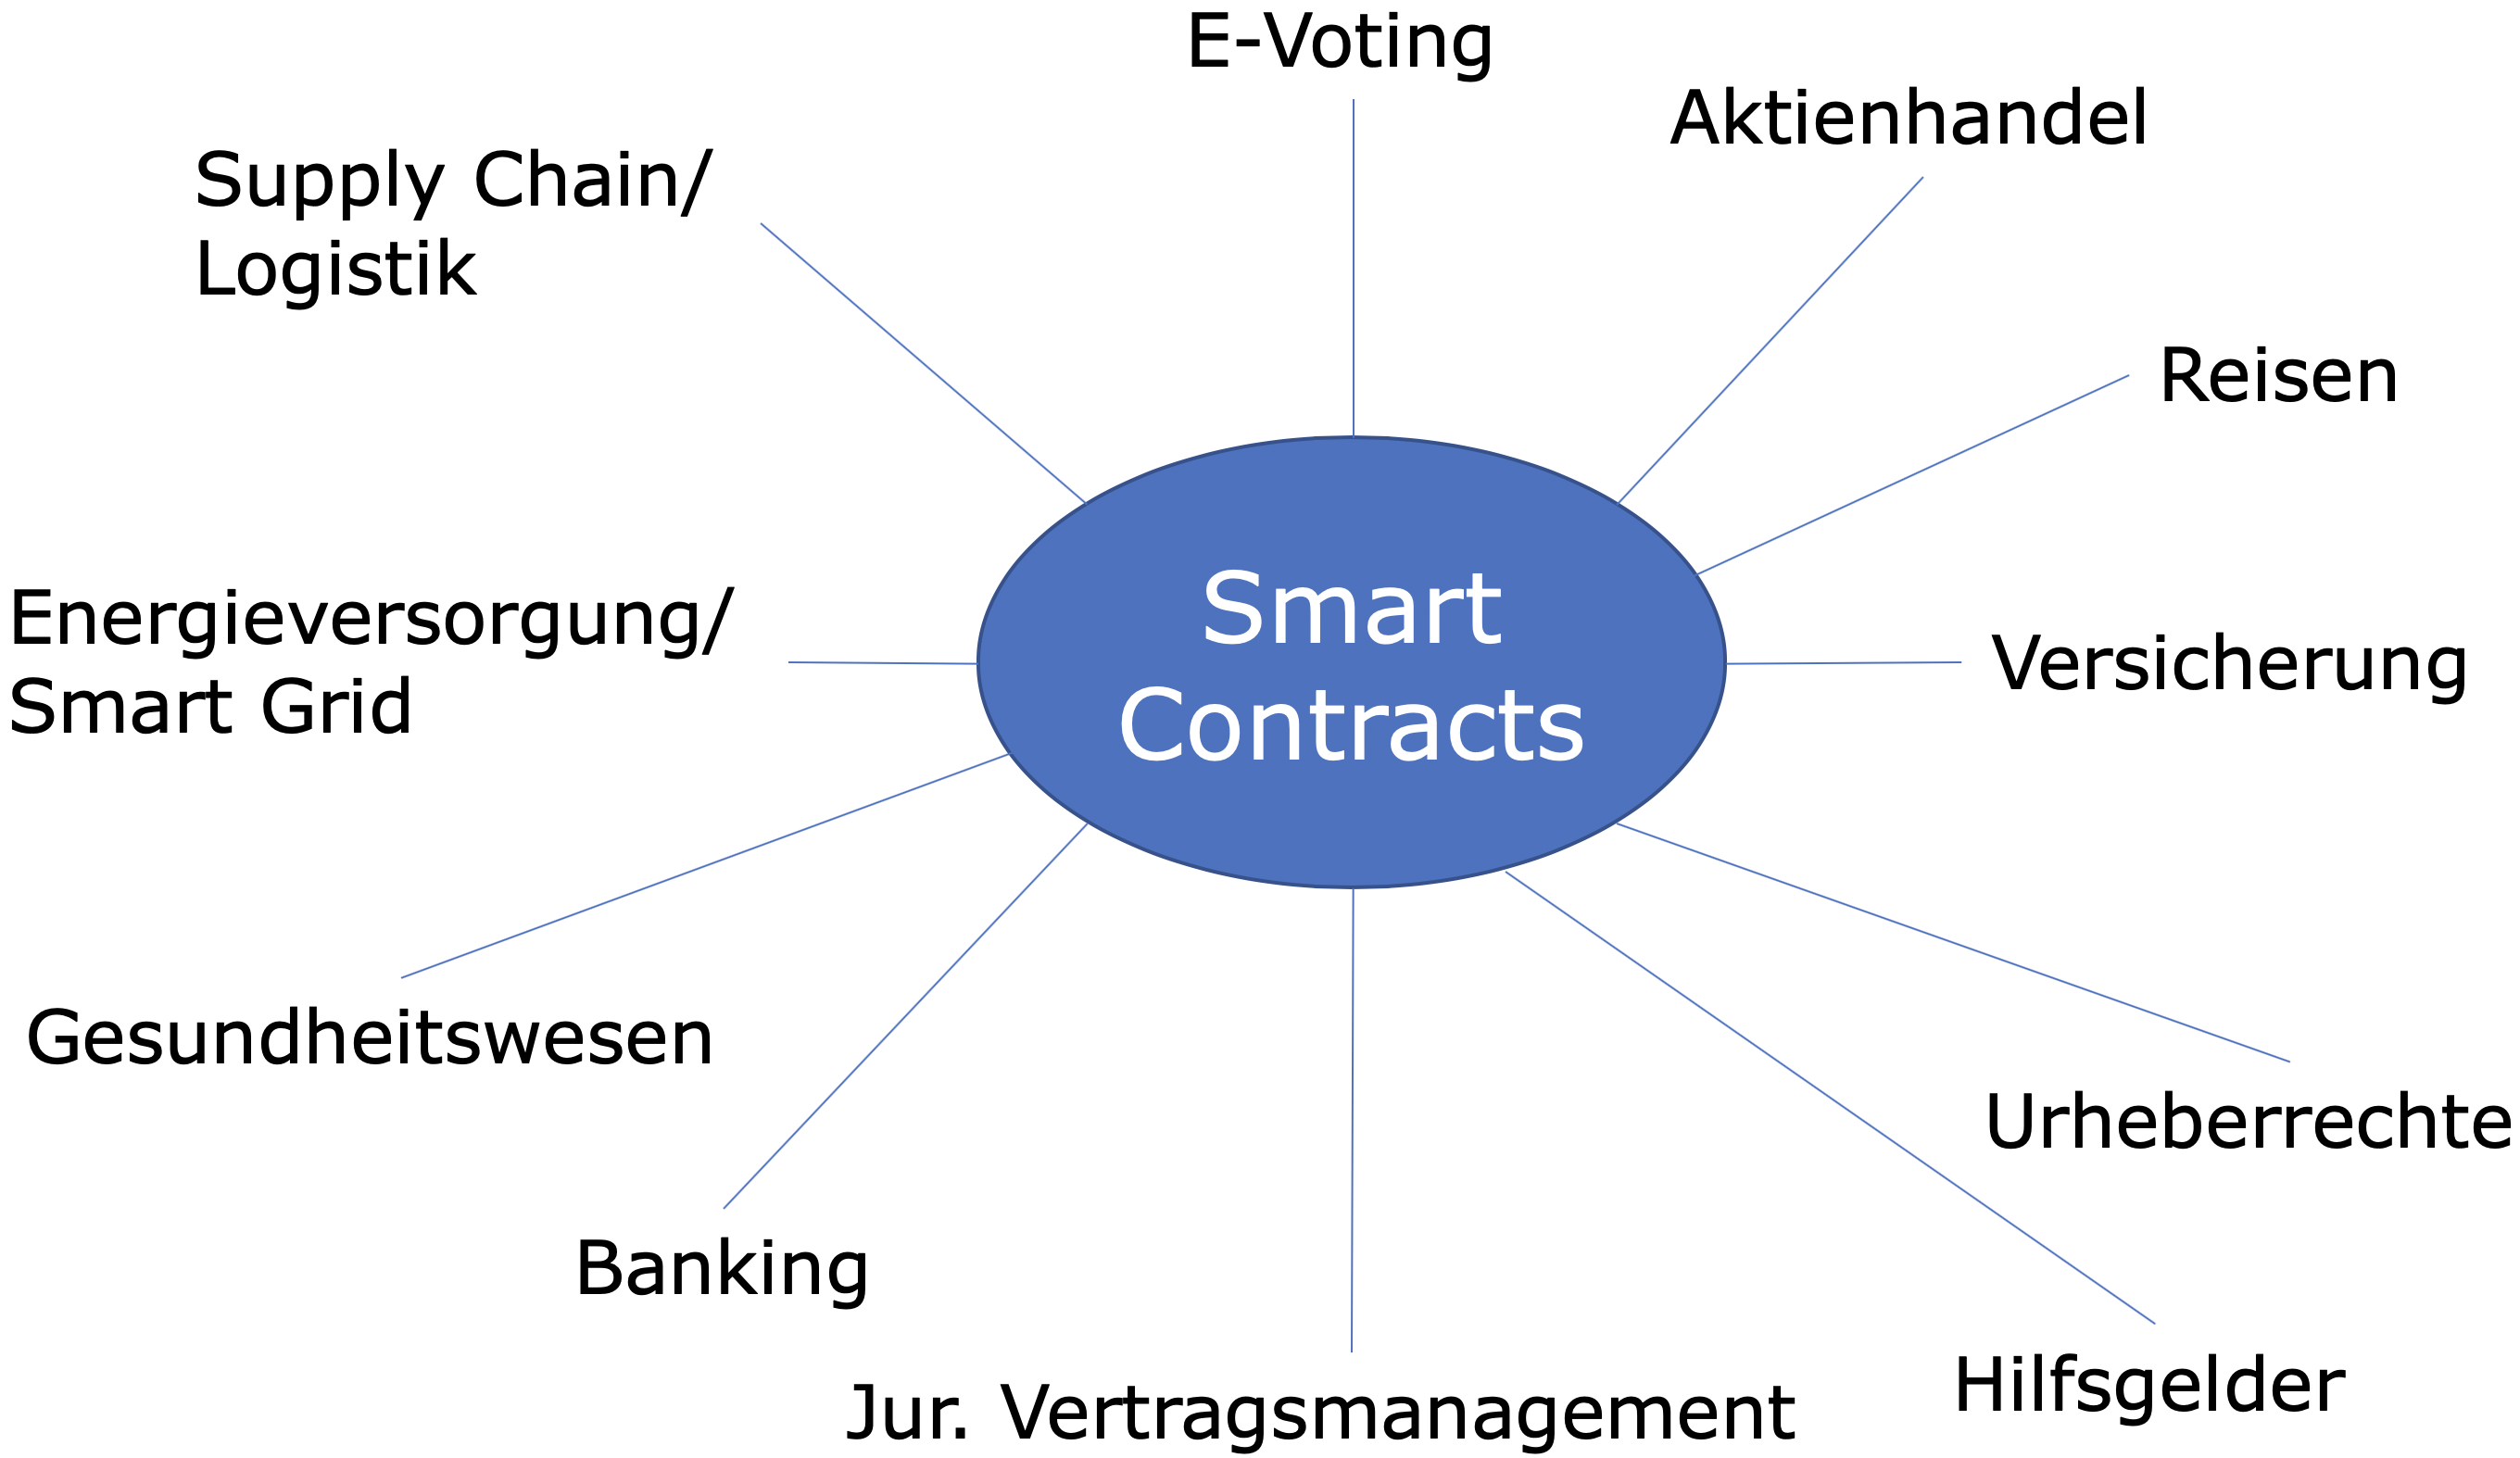
\includegraphics[width=\textwidth]{Bilder/Mindmap.png}
  \caption[Mindmap zu Smart Contracts]{Mindmap zu Smart Contracts (eigene Darstellung)}
  \label{fig:mindmap}
\end{figure}

Da es in dem geringen Umfang dieser Seminararbeit nicht möglich ist, im Detail auf alle Bereiche einzugehen, soll nun begründet dargelegt werden, wieso die jeweiligen Beispiele von der näheren Betrachtung ausgeschlossen wurden.\\ 

\textbf{E-Voting}\\
Generell ist das E-Voting ein Bereich, für den Smart Contracts prädestiniert scheinen \cite[vgl. z. B.][]{McCorry2017, Kshetri2018, Yavuz2018}. Die sichere, elektronische Abgabe von Stimmen, ist ein Thema, das viele Länder, darunter die Schweiz, beschäftigt. Diese gilt auf dem Fachgebiet seit Jahren als Pionier. Dort wurde 2018 das E-Voting in der Stadt Zug mittels Blockchain erfolgreich getestet \cite[vgl.][]{luxoft2018}. Mit Ökosystemen wie Agora wird zudem an alltagstauglichen Standards für die elektronische Stimmabgabe gearbeitet \cite[vgl.][]{Agora2019}. Trotzdem wird oftmals noch, wie in Deutschland, auf analoge Art und Weise abgestimmt. Ein Grund dafür stellt die Angreifbarkeit der Systeme dar. Daher wurde von der Schweiz die Offenlegung des Quellcodes und die Einrichtung eines Bug Bounty Programms beschlossen \cite[vgl.][]{Sperlich2019}. Überträgt man diese Gefahren auf die Blockchain, wird die Angriffsfläche durch solch eine basierte Lösung minimiert, generell sind Attacken aber nicht undurchführbar. \\
Aufgrund der allgemeinen Kontroverse über die Anwendung, sowie der Schwierigkeit, genaue Informationen über die eingesetzten Plattformen und Smart Contracts bei Blockchain-basierten Lösungen zu erhalten, wurde dieses Thema nicht zur genaueren Bearbeitung herangezogen.

\textbf{Aktienhandel}\\
Der Aktienhandel ist ein typisches Beispiel für zentralisierte Handelsplattformen. Mittels Smart Contracts und der Blockchain ließen sich an Transaktionen beteiligte Intermediäre entfernen und somit Kosten sparen \cite[vgl.][]{Notheisen2017}.\\
Eine komplett funktionierende Blockchain-Börse gibt es Stand heute nicht. Jedoch nähert sich zum Zeitpunkt des Verfassens dieser Arbeit mit SprinkleXChange die erste dieser Art ihrem Markteintritt \cite[vgl.][]{Hoikkala2019}.\\
Durch den frühen Stand der Implementierungen bzw. der Forschungskonzepte eignet sich dieses Thema nur bedingt für eine tiefe Begutachtung, weshalb es zugunsten anderer Themen nicht betrachtet wird.

\textbf{Urheberrechte}\\
Die Wahrung der Urheberrechte stellt in einer digitalen und globalisierten Welt eine große Herausforderung dar. Mit der umstrittenen EU-Reform um Artikel 13 respektive 17 sollte das Urheberrecht grundlegend erneuert werden \cite[vgl.][]{bpb2019}.\\
Musikverlage, wie Ujo Music, gehen mithilfe der Blockchain andere Wege und vertreiben über eine mehrschichtige Softwarearchitektur die Titel ihrer Künstler dezentral \cite[vgl.][]{Attar2018}. Nach ersten Tests ist die weitere Vorgehensweise jedoch unklar \cite[vgl.][S. 121 f.]{Gilli2019}.\\
Da auch hier die Entwicklungen der Industrie noch nicht absehbar und wenige konkrete Beispiele vorhanden sind, ist es nicht für diese Arbeit geeignet.

\textbf{Juristisches Vertragsmanagement}\\
Das klassische Vertragsmanagement, welches heute von einem Notar geführt wird, kann mittels Smart Contracts vereinfacht werden. Der Markt für Legal Techs, also Startups in der Rechtsbranche, scheint durchaus gegeben zu sein, da die Digitalisierung auch in diesem Bereich eine immer größere Rolle spielt. Eines davon ist die Firma TODO: [EINFÜGEN!!!!!!!!!]\\
Solange aber die rechtlichen Grundlagen für die Rechtssicherheit elektronischer Verträge in der Blockchain nicht gegeben sind, wird ihre Anwendung minimal sein.


\textbf{Banking}\\
Im Zuge der Recherche wurde der Kontakt zu Banken über öffentlich zugängliche E-Mail-Adressen gesucht. Da sich bis zum Zeitpunkt des Verfassens dieser Arbeit kein angeschriebenes Geldinstitut gemeldet hat, sind wenig verfügbare Informationen vorhanden. Allerdings zeigen Vorstöße, wie der von Wirecard \cite[vgl.][]{Weidemann2018}, dass es sich um ein durchaus interessantes Gebiet im Bankensegment handelt. Da Banken aber ohnehin darauf bedacht sein dürften, sensible Informationen wie z.B. Bankdaten nicht öffentlich zu speichern, wird in heutigen und zukünftigen Implementierungen von Smart Contracts wohl keine öffentliche Blockchain, wie beispielsweise Ethereum, herangezogen werden. \\
Das erschwert die Erlangung von Wissen über die eingesetzen Verfahren und Lösungen, weshalb Banking von den Themen ausgeschlossen wird.

\textbf{Gesundheitswesen}\\
TODO!!!

Somit verbleiben die Bereiche Reisen, Versicherung, Hilfsgelder, Energieversorgung/Smart Grid sowie Supply Chain/Logistik zur weiteren Begutachtung.
\chapter{Logistik}
\label{chap:Logistik}
Laut einer Bitkom-Studie aus dem aktuellen Jahr sehen 92 \% der befragten Logistikunternehmen eine Beschleunigung im Transport von Produkten mithilfe der Digitalisierung gegeben \cite{Bitkom2019}. Generell ist in der Branche zunehmen ein Drang nach Digitalisierung aufgrund der komplexen Prozessketten zu sehen. Wo in der Logistik Abmachungen zwischen Vertragsteilnehmern stattfinden, lassen sich Systeme auch ideal mittels Smart Contracts umsetzen. 

\section{Dachser}
Im Vorlauf zu dieser Arbeit und der dazugehörigen Präsentation konnte eine Besprechung mit einem fachkundigen Mitarbeiter der Firma Dachser aus Kempten durchgeführt werden. Seit 2016 wird dort in Zusammenarbeit mit dem Fraunhofer Institut an der Sinnhaftigkeit von Blockchain-Anwendungen sowie Smart Contracts und deren Use Cases geforscht. Dabei werden besonders zwei mögliche Systeme in Betracht gezogen: Hyperledger und Ethereum. Ziel ist es, die Technologie hinter den bekannt gewordenen Schlagworten zu verstehen.

\begin{figure}[h!]
  \centering
  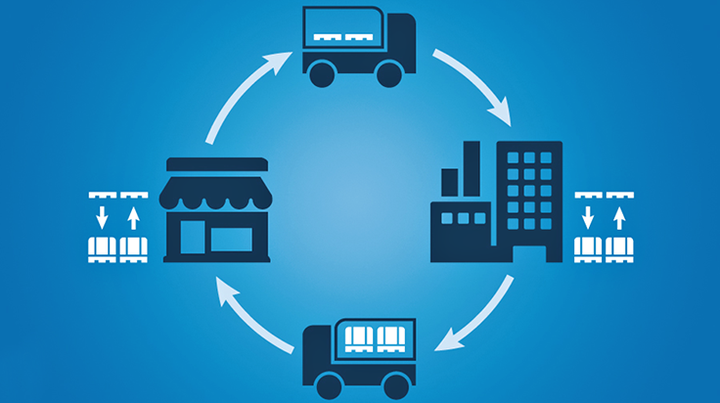
\includegraphics[width=\textwidth]{Bilder/Palettentausch.png}
  \caption[Palettentausch]{Palettentausch \cite{Disponaut2016}}
  \label{fig:palettentausch}
\end{figure}

Ein konkreter Anwendungsfall wurde im Rahmen einer Bachelorarbeit im Wintersemester 2018/2019 prototypisch umgesetzt. Dabei wurde exemplarisch der Palettentausch herangezogen. Diese Aufgabe stellt eine höhere organisatorische Hürde da als man anfangs vermuten würde. Betrachtet man das einfache Beispiel aus Abbildung \ref{fig:palettentausch}, sieht man einen immer wiederkehrenden Kreislauf. Sinn und Zweck des Palettentausch ist es, immer eins zu eins vollständig leere Europaletten gegen mit Ware beladene zu wechseln. Deshalb muss der Lastkraftwagen zunächst mit leeren Paletten beladen zum Produzenten fahren um dort die Ware zu beladen, welche er sodann zum Kunden transportiert. Dort angekommen erhält er wieder in gleicher Anzahl zur Lieferung leere Paletten. In der Praxis stellt sich das jedoch nicht als realistisches Szenario dar: Bei voller Beladung mit leeren Paletten muss immer noch genügend Platz für unpalettierte Ware vorhanden sein. Dadurch ist ein gleichmäßiger Palettentausch nicht durchsetzbar. Mittels oft nicht standardisierten Papierformularen, sogenannten Palettenscheinen, wird der Austausch zwischen den Geschäftspartnern quittiert. Sollte es zu einer ungleichmäßigen Verteilung kommen, wird ein Kontenbetrag von jedem Teilnehmer selbstständig abgebucht, um einen Ausgleich herzustellen. \cite[vgl.][]{Disponaut2016}

In der Zwischenzeit gab es eine Initiative der GS1, um den Palettenschein zu standardisieren und digitalisieren \cite[vgl.][]{GS12017}. Dadurch soll es auch möglich sein, ihn elektronisch untereinander auszutauschen. Ein Problem aber bleibt; die eigenhändige Abrechnung der beiden Parteien. Hier offenbart sich ein entscheidender Vorteil eines Smart Contracts. Da er die Kontostände der Teilnehmer kennt, kann er an zentraler Stelle die Schulden auf die jeweiligen Konten buchen. Dadurch fällt ein großer Teil der organisatorischen Komplexität weg. So wurde es auch in einem Proof of Concept in der oben genannten Bachelorthesis gezeigt, welcher aber nie im Produktionsmodus angewandt wurde.

Allgemein hat sich bei der Firma Dachser herausgestellt, dass die Blockchain und die darunterliegenden Smart Contracts nicht unter den aktuellen Gegebenheiten als sinnbringende Technologien eingesetzt werden können. Damit es eine praktikable Lösung darstellt, müssten weitere Industriepartner in die Blockchain eingebunden werden, darunter auch direkte Konkurrenten der Firma Dachser, wie beispielsweise DB Schenker. Per Definition kann nun jeder die Transaktionen, welche bei einem Smart Contract anfallen, nachvollziehen. Wollte man die Sichtbarkeit untereinander einschränken, müsste man die Blockchain so abändern, dass sie im Endeffekt nicht mehr ihrer eigentlichen Bestimmung gerecht wird. In der Branche wird ein Umdenken gefordert, damit nützliche Modelle nicht an der Umsetzung scheitern müssen. Letztendlich hängt ein Großteil nicht an der Technik, sondern an der unternehmenspolitischen Ausführung.\\
Ein weiteres Manko ist das Fehlen von Standards bei der Implementierung von Smart Contracts, da sie nicht im Nachhinein vom Programmierer abgeändert werden können. Das sorgt zusehends für Verwirrung und Ungereimtheiten bei der Implementierung, was bei klassischen Systemen durch Industrie- und Programmierstandards nahezu ausgeschlossen werden kann. Oftmals stellt sich eine herkömmliche Lösung als einfacher und tragfähiger heraus, besonders dort, wo sowieso nur ein Server/Node benötigt wird, was die dezentrale Implementierung in einer Blockchain obsolet macht.\\
Betrachtet man die heutigen Anforderungen an den Datenschutz im Unternehmen, so steht die Speicherung in einer Blockchain unter Umständen in klarem Kontrast du den Forderungen der Datenschutzgrundverordnung. Diese fordert eine Löschbarkeit bzw. Anonymisierung der Daten bei Erstellung respektive im Nachhinein. Durch die Unveränderlichkeit der Blockchain ist das schlichtweg nicht durchführbar. Die aktuell vorherrschenden Gesetze bieten keine Möglichkeit, Probleme wie den Palettentausch mit Palettenschein sinnvoll auf einen Smart Contract abzubilden.

\section{Tradelens}
Eine erfolgreich im Markt bestehende Softwarelösung ist Tradelens, ein Produkt, welches in Kooperation von IBM und der dänischen Reederei Maersk entstanden ist. Das Ziel ist, eine Plattform für möglichst viele Beteiligte zu liefern, um damit an der Spitze der digitalen Transformation in der Logistik zu stehen \cite[vgl.][S. 7]{Tradelens2019b}. Tradelens besteht aus insgesamt drei Ebenen: Netzwerk, Plattform und Applikationen (siehe Abbildung \ref{fig:tradelensOverview}).

\begin{figure}[h!]
  \centering
  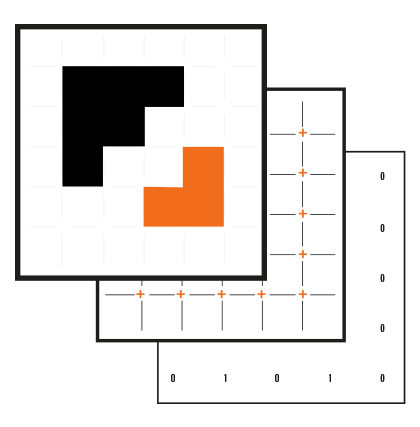
\includegraphics[width=.4\textwidth]{Bilder/Tradelens-Overview.png}
  \caption[Tradelens Aufbau]{Tradelens Aufbau \cite{Tradelens2019a}}
  \label{fig:tradelensOverview}
\end{figure}

\textbf{Netzwerk}\\
Das Netzwerk bildet die Grundlage von Tradelens. Formal beschrieben umfasst es alle Business-Teilnehmer, welche an dieser spezifischen Blockchain-Lösung teilnehmen. So ist es möglich, die Teilhabenden an der gesamten Supply-Chain abzudecken. Dies reicht von den Verschiffern, über Versandunternehmer bis zu Regierung und das zuständigen Zollbüro. Die anfallende Menge an Informationen und Daten kann genutzt werden, um den gesamten Lebenszyklus einer Lieferung nachvollziehen zu können. \cite[vgl.][S. 5]{Tradelens2019b}

\textbf{Plattform}\\
Plattformseitig zählt Tradelens nicht zu einer Ethereum basierten Lösung. Vielmehr wird auf Hyperledger Fabric aufgesetzt. Das ist eine ursprünglich von IBM entwickelte und an die Linux Foundation gespendete Applikation. Heute existiert mit Hyperledger bereits ein ganzes Ökosystem rund um Software der Blockchain. Diese Plattform bietet vielfältige Möglichkeiten zum Dokumentenaustausch. Wie im vorigen Beispiel bei Dachser angesprochen, lässt sich zeigen, dass noch viele Abläufe der Logistik papierbasiert abgewickelt werden. Tradelens bietet hiermit nicht nur eine hohe Automatisierungsrate für Rechnungen, Packlisten, Buchungsbestätigungen etc., sondern liefert auch standardisierte Formulare. Werden diese Vorgänge abgeschlossen, setzen die Smart Contracts an, um einen reibungslosen Ablauf gewährleisten zu können. Um das Vertrauen der Kunden aufrecht erhalten zu können, wird eine Berechtigungsverwaltung eingesetzt, damit nur an einer Transaktion beteiligte Partner Informationen abrufen können. Zusätzlich sind alle Daten generell verschlüsselt abgelegt. \cite[vgl.][S. 11 ff.]{Tradelens2019b}

\textbf{Applikationen}\\
Auf der letzten Ebene liegen die Applikationen. Tradelens an sich bietet nur einen gewissen Grundstock an Funktionalität. Will man Schnittstellen zu speziellen Systemen herstellen, oder Tradelens um spezifische Fähigkeiten erweitern muss das selbst erfolgen. Daher kann auch jedermann auf einem extra dafür bereitgestellten Marktplatz Applikationen an potentielle Kunden anbieten. Durch diesen Austausch können die Teilnehmer untereinander von den Entwicklungen der anderen profitieren. Tradelens will eine offene Lösung herstellen, welche man selbst nach Belieben erweitern und an seine Vorstellungen anpassen kann. \cite[vgl.][S. 5]{Tradelens2019b}

Versucht man, genauere Informationen über die zugrundeliegende Plattform und die eingesetzten Smart Contracts zu erhalten, kommt man schnell an die Grenzen des Systems. Das ist natürlich einerseits so gewollt, damit die sensiblen Daten der Plattformteilnehmer nicht in fremde Hände geraten, andererseits ist der Grundgedanke einer Blockchain wahrlich ein anderer. Es wird zwar mit einer offenen Plattform geworben -- das mag durchaus legitim sein -- dennoch wird die Open Source Blockchain Hyperledger Fabric so verändert, dass sie nicht mehr einer Blockchain entspricht. Letztendlich kommt es zu einem geschlossenen System, welches in der Hand von einigen wenigen Unternehmen liegt. So ist es kaum verwunderlich, dass ein IBM-Account benötigt wird, um nur grundsätzliche Informationen abzurufen. Das Beobachten von Transaktionen oder gar den Contracts ist schlichtweg als Nichtteilnehmer nicht möglich.

\section{Weitere Beispiele}
In der Logistik bestehen noch weitere prestigeträchtige Beispiele für den Einsatz von Blockchain und Smart Contracts, auf die bisher noch nicht eingegangen wurde. Eines davon ist die Lebensmittel Blockchain des US-Supermarkts Walmart. Dort wurde eine Hyperledger Fabric Lösung mithilfe IBM entwickelt, um eine bessere Nachverfolgbarkeit von Lebensmitteln gewährleisten zu können. Kommt es zu Epidemien aufgrund verseuchter Lebensmittel, lässt sich der Ursprung der Produkte in Sekundenschnelle bestimmen. Ein Vorgang der früher mit bis zu sieben Tagen deutlich komplexer zu bewerkstelligen war. \cite[vgl.][]{Hyperledger2019}\\
Mit Cobility findet sich eine weitere Initiative, um ein dezentrales System in der Logistikbranche zu etablieren. Tiefergehende Informationen sind auch hier leider nicht zu erhalten, da ein geschlossenes System der Firma evan.network verwendet wird. Durch die Unterstützung vieler großer Industriepartner wirkt das System jedoch sehr prestigeträchtig. Innerhalb des zweiten Quartals diesen Jahres wird die erste Anwendung freigeschalten, wozu zuvor noch Rahmenbedingungen definiert wurden. Langfristig soll das System weiter ausgebaut werden und weiter wachsen. Da Cobility ein Gemeinschaftsprojekt dreier deutscher Firmen ist, steht es in direkter Konkurrenz zu Lösungen wie beispielsweise Tradelens. Da der Reifegrad dieser Lösung aber noch nicht so weit fortgeschritten ist, ist es fraglich, inwieweit sie sich gegen Konkurrenzsysteme durchsetzen kann. \cite[vgl.][]{Cobility2019}
\chapter{Reisebranche}
\label{chap:Reisebranche}
Die Reisebranche wird von wenigen Anbietern auf dem Markt bedient, was zu einem sogenannten Oligopol führt. Betrachtet man den größten Reiseportalbetreiber in Deutschland aus dem Jahr 2017, Booking.com, so fällt auf, dass er hierzulande mit weitem Abstand die Liste der umsatzstärksten Unternehmen in diesem Bereich anführt \cite[vgl.][]{FVW2017}. Das ist nicht verwunderlich, vereint die Booking Holding unter sich auch Marken wie Agoda, Momondo oder Kayak \cite[vgl.][]{Booking2019}. Beim zweitgrößten Betreiber Expedia verhält es sich ähnlich; auch hier gibt es Tochterfirmen wie Trivago, Homeaway und Ebookers \cite[vgl.][]{Expedia2019}.\\
Aufgrund des geringen Marktdrucks der Anbieter werden häufig veraltete IT-Systeme eingesetzt, welche zu Sicherheitslücken neigen. Im Jahr 2017 kam es so beispielsweise zu Hackerangriffen auf das Computerreservierungssystem von Sabre, einer der Top drei Firmen auf diesem Gebiet \cite[vgl.][]{Mathews2017}.

Um das Missverhältnis zwischen Angebot und Nachfrage auszugleichen sowie eine Erneuerung der IT anzustreben, engagieren sich Firmen wie Winding Tree, um mittels Blockchain und Smart Contracts eine direkte Verbindung zwischen Airlines bzw. Hotels und den Buchenden herzustellen (siehe Abbildung \ref{fig:windingTreeOverview}). Um die Notwendigkeit dazu zu untermauern hebt Winding Tree in ihrem Whitepaper als Ausgangspunkt vor allem die hohen Gebühren hervor, die die klassischen Intermediäre bei erfolgreicher Vermittlung berechnen \cite[vgl.][S. 2 f.]{WT2019}.

\begin{figure}[h!]
  \centering
  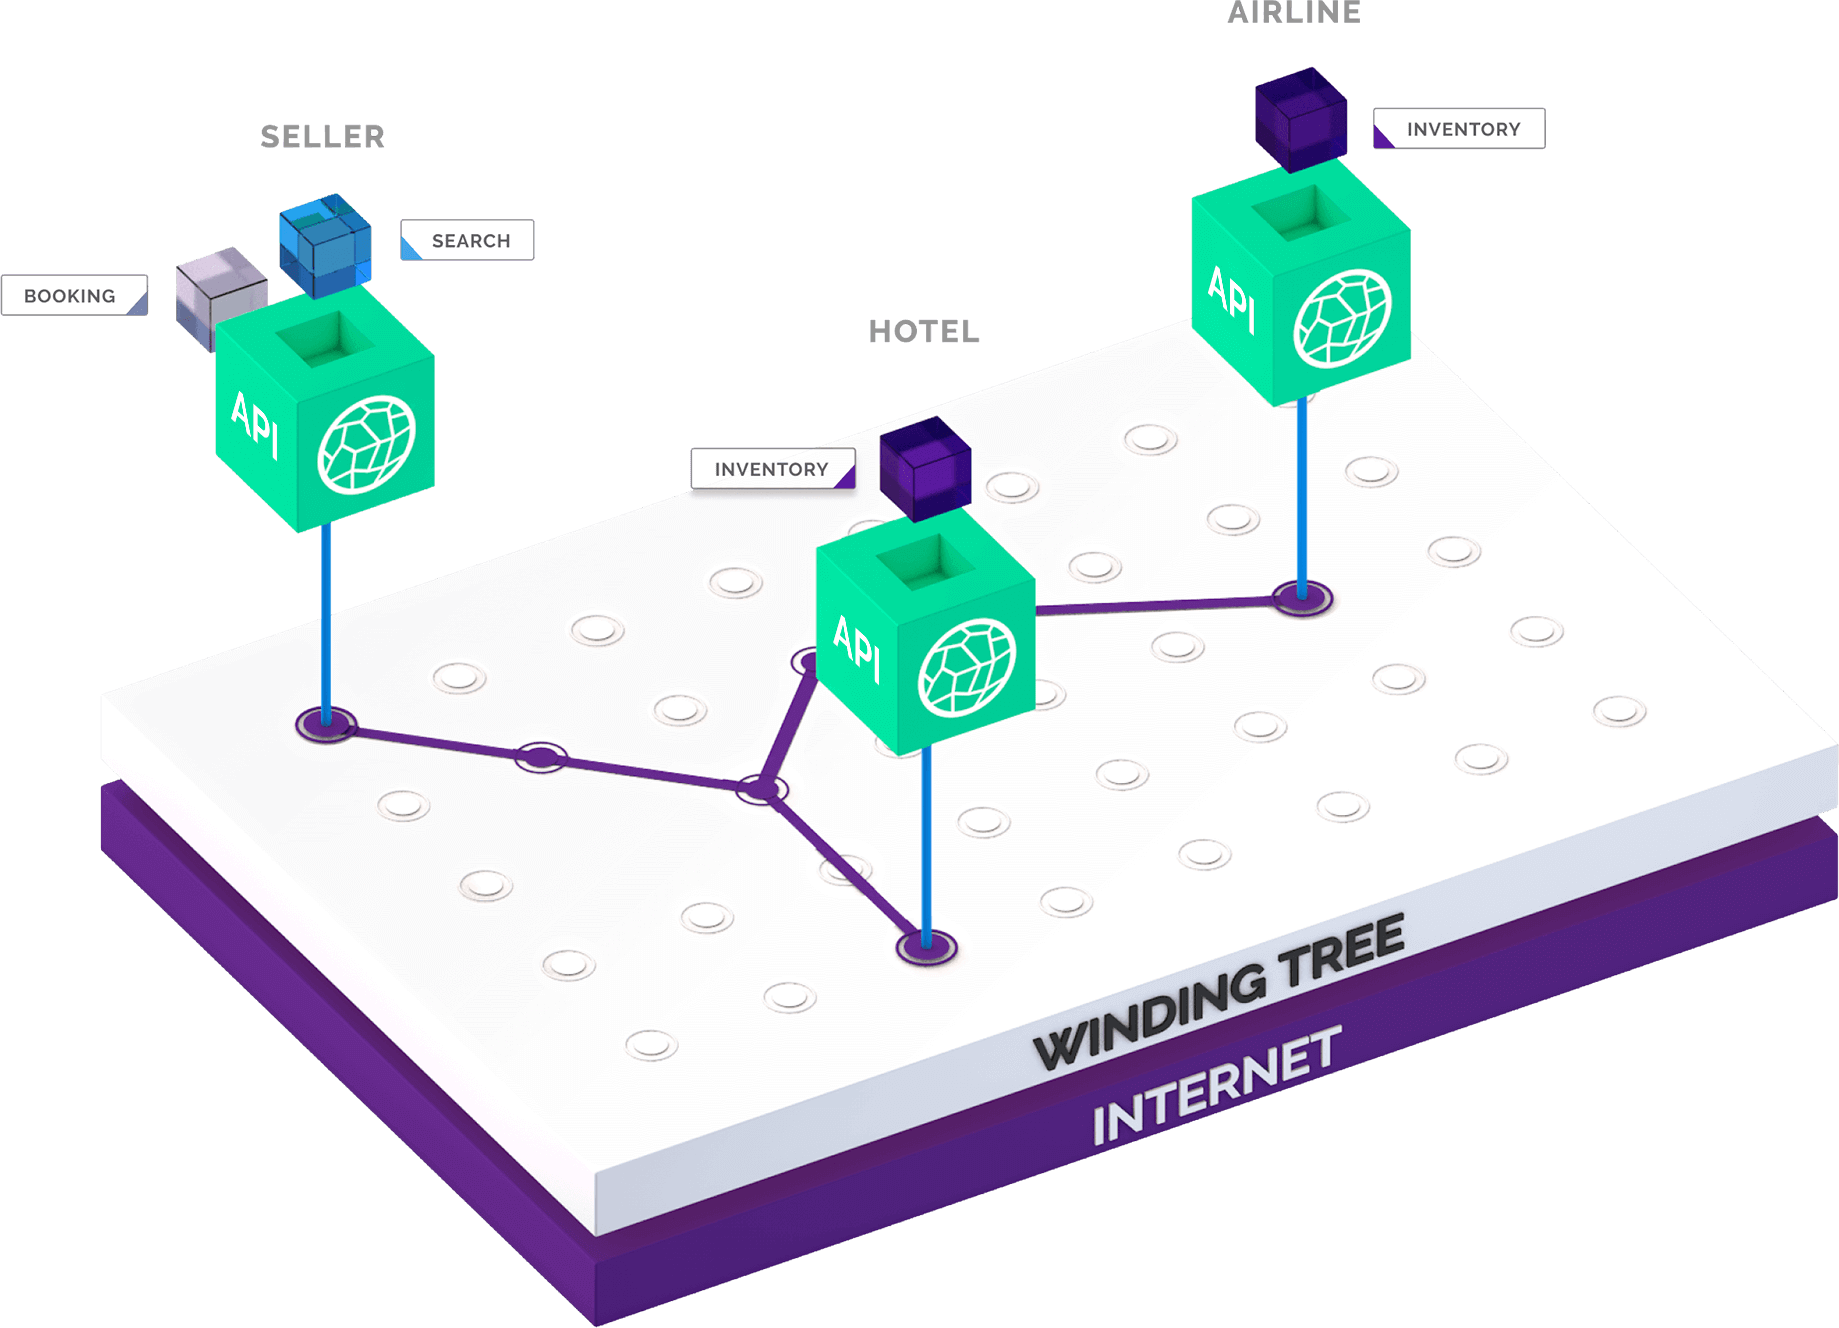
\includegraphics[width=\textwidth]{Bilder/WindingTreeOverview.png}
  \caption[Winding Tree Überblick]{Winding Tree Überblick \cite{WTWebsite2019}}
  \label{fig:windingTreeOverview}
\end{figure}

Winding Tree bietet lediglich die Plattform inklusive Schnittstellen zur Abwicklung der Geschäftsbeziehungen an, alle weiteren Anwendungen (z. B. Benutzeroberflächen) müssen von den Teilnehmern selbst implementiert werden. Dabei stehen als Hilfestellung allerdings auch Referenzimplementierungen in JavaScript unter der Apache-2.0-Lizenz auf Winding Trees GitHub Account bereit \cite{WTGitHub2019}.\\
Dass dies nicht nur eine Nischenlösung ist, wird beim Blick auf die Industriepartner bewusst: Neben Hotelketten wie Nordic Hotels sind vor allem große europäische Airlines auf der Plattform vertreten. Dazu gehören unter anderem auch AirFrance, KLM, SWISS, Eurowings und die Lufthansa \cite{WTWebsite2019}.

Eigens für die Plattform wurde der Líf Token generiert, welcher mehr Daten als ein typischer ERC20 Token verarbeiten kann und dabei die Kompatibilität beibehält \cite[][S. 9]{WT2019}. Dadurch können die für Reisen benötigten Daten kostengünstiger verarbeitet werden.\\ 
Zudem ergibt sich der Nebeneffekt der Plattformfinanzierung, was 2018 in Form eines Token Generation Events umgesetzt wurde. In mehreren Stadien konnten Ether in Líf umgewandelt werden. In der ersten Woche wurden 1000 Líf je Ether ausgeschüttet, in der zweiten Woche noch 900. Dabei wird die Anzahl der generierten Token vom Markt bestimmt. Stand heute (26. Juni 2019) ist ein Líf zum Preis von 0.0003 ETH respektive 0.91831 Eurocent erhältlich \cite{Coinmarketcap2019}. Um die laufenden Kosten für die Entwicklung der gemeinnützigen Firma Winding Tree tragen zu können, wurde zudem ein Marktvalidierungsmechanismus eingebaut. Dieser ist in Form eines autonomen Smart Contracts angelegt, welcher die Kapitalisierung, die die Marke von umgerechnet zehn Millionen US-Dollar zum Token Generation Event überschritten hat, verwaltet. Anhand einer festgelegten Preisfunktion werden Token angekauft und direkt vernichtet. Heute (Stand 26. Juni 2019) werden dort noch 4189 Ether, umgerechnet mehr als eine Million Euro, vorgehalten \cite{Lif2019}. Anhand [vgl.][S. 12 ff.]{WT2019}. \\
Somit gilt Líf als Wertinstrument für alle abzuwickelnden Tätigkeiten, die auf dem System stattfinden sollen. Am besten wird das am Beispiel aus Abbildung \ref{fig:windingTreeExample} deutlich.\\

\begin{figure}[h!]
  \centering
  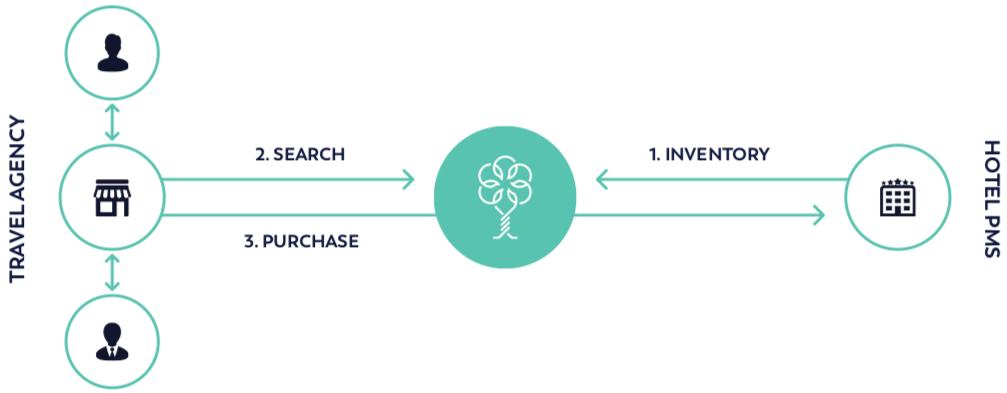
\includegraphics[width=\textwidth]{Bilder/WindingTreeExample.png}
  \caption[Beispiel eines Geschäftsfalls]{Beispiel eines Geschäftsfalls \cite[S. 10]{WT2019}}
  \label{fig:windingTreeExample}
\end{figure}

Um aus dem Property Management System des Hotels freie Zimmer an Winding Tree zu melden, muss eine zu diesem Zeitpunkt berechnete Menge an Líf gezahlt werden. Betrachet man die Smart Contracts und die API-Implementierungen aus dem oben bereits genannten GitHub Account, wird nicht sofort ersichtlich, wie diese Inventur getätigt wird. Die Contracts für die Airlines und Hotels sind relativ kurz gehalten und beschränken sich auf das Nötigste. Im Fall von Änderungen werden daher in der Regel nur Daten im Byteformat übertragen. Um die Zugriffe auf den Contract zu kapseln, und damit einfacher zu gestalten, dienen die angesprochenen APIs, welche in \emph{booking}, \emph{notification}, \emph{write} und \emph{read} unterteilt sind \cite[vgl.][]{WTAPIOverview2019}.\\
Um solche Änderungen einzupflegen müsste über den Contract zuerst ein Hotel im System angelegt werden. Dazu dient die Methode \texttt{registerHotel(...)}. Diese bindet das Hotel an einen \emph{manager}, der jedoch mittels \texttt{transferHotel(...)} das Hotel an eine andere Adresse übertragen kann. Über die \emph{write}-API werden schlussendlich die Daten des Hotels über die Methode \texttt{callHotel(...)} des Hotels überschrieben. \cite[vgl.][]{WTHotelContract2019, WTInventory2019}\\
Nun ist das Hotel für eine etwaige Reiseagentur über die Plattform auffindbar. Diese kann per \emph{read}-API potentielle Hotels abrufen. Momentan werden die Hotels in der Reihenfolge, wie sie in den Winding Tree Index geschrieben worden sind, ausgegegen. Somit lässt sich auch erst einmal nicht nach Hotels in der gewüschten geographischen Lage filtern, was durchaus problematisch werden könnte, wenn man kein Hotel als möglichen Kandidaten ausschließen will. Jedoch können unnötige Informationen über die Hotels auch mithilfe des Requests entfernt werden, d.h. z.B. lediglich die Blockchain-Adresse und die Koordinaten angezeigt werden, womit aber nicht das Problem des Abrufens letztendlich aller Hotels des Indexes gelöst wird. \cite[vgl.][]{WTQueryInventory2019}\\
Ist ein passendes Hotel gefunden, kann es gebucht werden. Dafür wird die \emph{booking}-API verwendet. Neben den Informationen über Gäste müssen auch Preisinformationen angefügt werden. Diese können aus den Daten der Plattform berechnet werden. Wieso die Daten nicht innerhalb eines Contracts beigefügt werden, ist unklar. \cite[vgl.][]{WTBooking2019}\\
Um auf Hotelseite die Buchung zu akzeptieren, muss eine sogenannte \texttt{bookingUri} hinterlegt sein. Um das einzutragen, sei an dieser Stelle auch wieder auf die \texttt{callHotel(...)}-Methode des dazugehörigen Smart Contracts verwiesen. Die URI zeigt auf ein hotelinternes System, welches eine REST API aufspannt, welche wiederum die Buchungsschnittstelle abbildet. An den Endpunkten der Schnittstelle kann dann eine Buchung hinterlegt, bzw. im Zweifelsfall storniert werden. \cite[vgl.][]{WTBookingAccept2019}

Als Abschluss dieses Kapitels sollen nochmals kurz einzelne Punkte aufgegriffen werden.\\
Positiv anzumerken ist das Verfügbarmachen aller Implementierungen. Von den Contracts bis hin zu den Schnittstellen-Implementierungen kann alles nachvollzogen werden. Bei Bedarf besteht die Möglichkeit, tiefer in das System einzusteigen. Ob jedoch die Öffnung des Quellcodes zu mehr Sicherheit beiträgt, ist umstritten. Die Möglichkeit, auf Schwachstellen aufmerksam machen zu können, ist dennoch hervorzuheben und bekräftigt die Ausrichtung Winding Trees zu offenen Softwaresystemen, wie der Ethereum Blockchain. Durch namhafte Kooperationen und eine im Voraus geplante Finanzierung, ist diese Smart Contract Anwendung durchaus als ernsthaft und positiv zu betrachten.\\ 
Dennoch wird aus den Reihen der Reisebranche auch Kritik laut.

%- Líf-Token -> Notwendigkeit, Grundlage, ganz kurz Token Event; Market Validation Mechanism interessanter [Seite 2 und 3 halb] \\ % https://windingtree.com/White_Paper_EN.pdf
%- Ablauf allgemein (Beispiel aus Whitepaper) + Contracts genauer (siehe GitHub) [Seite 3 halb und 4]\\#
%- Kritik am System [Seite 4] \\
\chapter{Versicherung}
\label{chap:Versicherung}
Im Bereich Versicherung gibt es mehrere Bestrebungen, mithilfe von Smart Contracts die automatische Abwicklung von Versicherungsfällen zu regeln. Die 2018 gegründete B3i Initiative, hinter der namhafte Versicherungsunternehmen wie Zurich, AXA, Generali und die Allianz stehen, hat sich zur Aufgabe gemacht, Standards für die Branche zu entwickeln und das nötige Netzwerk und die Anwendungen aufzubauen \cite[vgl.][]{B3iWhoWeAre2019}. Da die Applikation erst im Juli 2019 startet \cite[vgl.][]{B3iHackathon2019}, eignet es sich nicht, um tiefer darauf einzugehen.

Eine bereits lauffähige Anwendung auf der Ethereum Blockchain existiert mit fizzy, einer Applikation von AXA. Fizzy sichert Personen gegen Flugzeugverspätungen bei mehr als zwei Stunden oder kompletter Annulierung des Fluges ab. Mit Anlegen einer Versicherung, was bis spätestens fünf Tage vor Abflug möglich ist, wird die Fluginformation an einen Smart Contract weitergegeben, welcher die Daten in der Blockchain speichert. Durch eine Koppelung an Flugdaten wird der Betrag im Versicherungsfall innerhalb einer Standard-Bankenlaufzeit ausbezahlt. Die Gebühren für die Absicherung werden dabei von einem Algorithmus anhand des Flug-Ausfallsrisikos berechnet. Durch den Einsatz von Blockchain-Technologie wird auf beiden Seiten Transparenz und Unveränderlichkeit der Bedingungen garantiert. \cite[vgl.][]{Fizzy2019}

Da fizzy mit \cite{Clement2019} einen Artikel bereitgestellt hat, um einen besseren Einblick in den zugrundeliegenden Smart Contract zu bekommen, wird im Folgenden ein Beispiel besprochen.\\
Seit 22. Mai 2019 gibt es eine neue Variante des Smart Contracts \cite{EtherscanNewContract2019}, welcher mit 742 Zeilen Solidity Code deutlich mehr Funktionalität liefert, als der ursprüngliche Smart Contract mit gerade einmal etwas mehr als 200 Codezeilen \cite{EtherscanOldContract2019}. Zur Betrachtung wird nun in Teilen der neue Contract herangezogen.

Die Schritte (1) und (5) aus Abbildung \ref{fig:fizzyAblauf} können vernachlässigt werden, da sie sich nur mit der Eingabe der persönlichen Daten und Flugdetails beschäftigen und der letzendlichen Kompensation im Versicherungsfall dienen. Interessanter sind hier die Schritte (2), (3) und (4), welche sich direkt mit dem Smart Contract beschäftigen. Nach diesen wird jeweils die Funktion \texttt{InsuranceUpdate(...)} im Nachgang aufgerufen.\clearpage

\begin{figure}[h!]
  \centering
  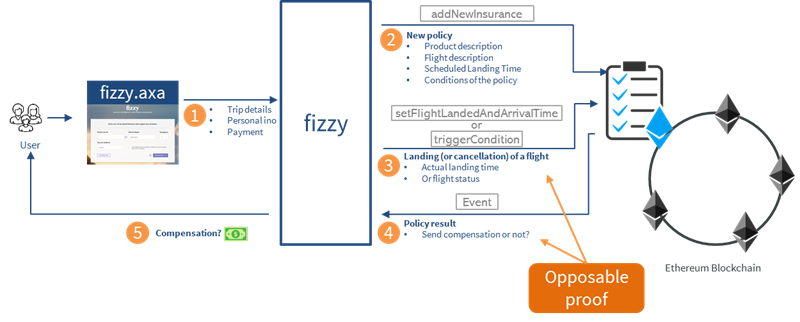
\includegraphics[width=\textwidth]{Bilder/fizzyAblauf.png}
  \caption[Ablauf fizzy Smart Contract]{Ablauf fizzy Smart Contract \cite{Clement2019}}
  \label{fig:fizzyAblauf}
\end{figure}

Anfangs muss eine Versicherung angelegt werden. Dafür steht die Solidity-Funktion \texttt{addNewInsurance(bytes32 flightId, uint256 productId, uint256 premium, uint256 indemnity, uint256 limitArrivalTime, uint256 conditions)} bereit. Kurz zur Erläuterung der einzelnen Parameter:

\begin{itemize}
    \item \texttt{flightId}: In Hexadezimal-Darstellung steht die Flugnummer inklusive Abflugdatum (UNIX-Timestamp) bereit
    \item \texttt{productId}: Identifikator, um Versicherung eindeutig zu kennzeichnen; es können auch mehrere Versicherungen mit der gleichen \texttt{flightId} existieren
    \item \texttt{premium}: Prämienbetrag, hexadezimal codiert
    \item \texttt{indemnity}: Entschädigung, hexadezimal codiert
    \item \texttt{limitArrivalTime}: spätester Ankunftszeitpunkt, d.h. geplanter Ankunftszeitpunkt + 2 Stunden (UNIX-Timestamp, UTC)
    \item \texttt{conditions}: binär kodierte Konditionen; 1001 (2) = 9 (10): für Verspätung und Canceln abgesichert, 0001 (2) = 1 (10): nur für Canceln abgesichert
\end{itemize}

Aus dem Contract wird die Transaktion\\
\texttt{0x6ecc9789935ff5c518f44fa9b2601f40ac6a8a4fa45f16f21146251dc9c9536a} beispielhaft ausgewählt. Die zugehörigen Werte obiger Funktion sind in Abbildung \ref{fig:fizzyNewInsurance} zu sehen.

\begin{figure}[h!]
  \centering
  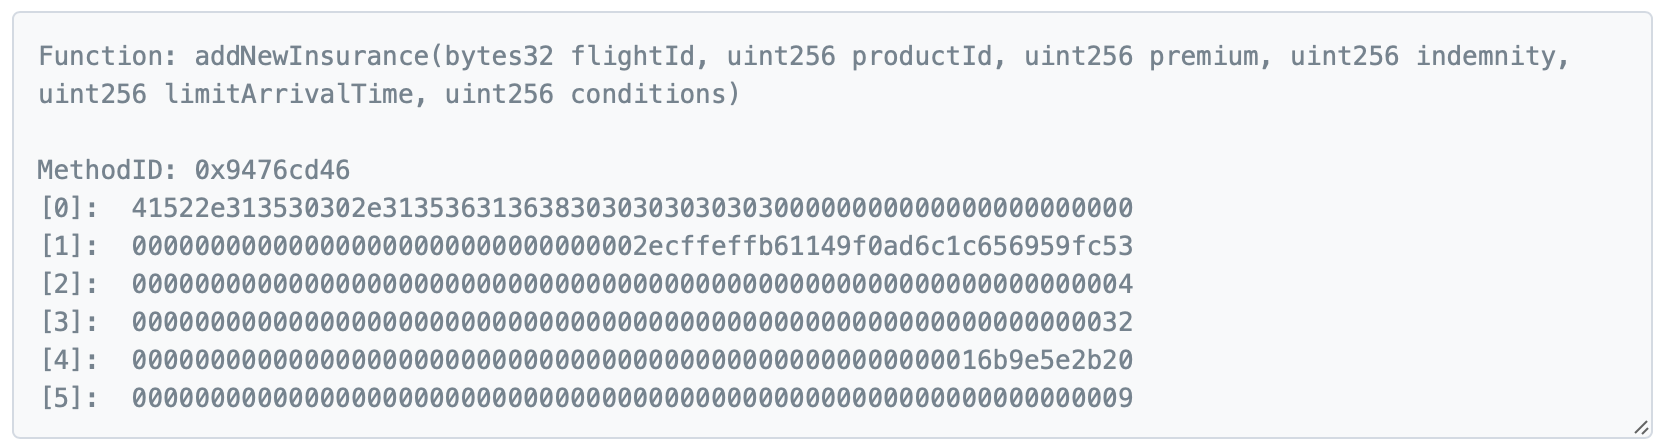
\includegraphics[width=\textwidth]{Bilder/FizzyExampleNewInsurance.png}
  \caption[Input-Daten addNewInsurance]{Input-Daten addNewInsurance \cite{FizzyNewInsurance2019}}
  \label{fig:fizzyNewInsurance}
\end{figure}

Mithilfe eines Hexadezimal zu String Decoders lässt sich die \texttt{flightId} zu \\ \texttt{AR.1500.1561680000000} umwandeln. Dabei beschreibt \texttt{AR.1500} den Flug, was sich nach einer Suchmaschinen-Recherche als Reise von Buenos Aires nach Córdoba mit der Fluggesellschaft Aerolineas Argentinas herausstellt. \texttt{1561680000000} ergibt mit einem UNIX-Timestamp-Converter den 28. Juni 2019. Auch die Hexadezimalen Werte der Prämien- und Entschädigungsbeträge lassen sich einfach umwandeln. So kommt man auf eine Prämie von 4€ sowie eine mögliche Entschädigung in Höhe von 50€. Die limitierte Ankunfszeit liegt am 28. Juni 2019 um 13:55 (GMT). Der Versicherte hat sich sowohl gegen Verspätung als auch gegen Ausfall abgesichert.

\begin{figure}[h!]
  \centering
  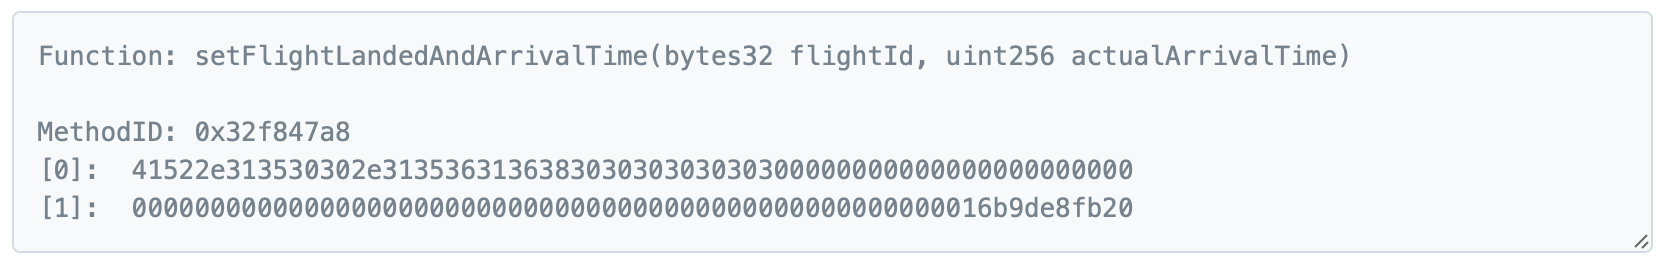
\includegraphics[width=\textwidth]{Bilder/FizzyExampleFlightLanded.png}
  \caption[Input-Daten setFlightLandedAndArrivalTime]{Input-Daten setFlightLandedAndArrivalTime \cite{FizzyFlightLanded2019}}
  \label{fig:fizzyFlightLanded}
\end{figure}

Sieht man in einem Tool wie etherscan.io in die Transaktionsliste, findet man am 28. Juni die Transaktion \texttt{0xcb63f57039f144073c4a4b45621a3c0da4593bd2185c14838d7b7e4c537f5be9}, deren Daten auch in Abbildung \ref{fig:fizzyFlightLanded} zu sehen sind. Da die tatsächliche Ankunftszeit mit umgerechnet 11:47 (GMT) weit unter der Höchstgrenze liegt, wird in diesem Fall keine Kompensation ausgezahlt.\\
Anders im Beispiel aus Abbildung \ref{fig:fizzyTrigger}, bei dem der Status auf 1 gesetzt wird, was gleichzusetzen mit einem abgeschlossenen Flug inklusive Kompensation ist.

\begin{figure}[h!]
  \centering
  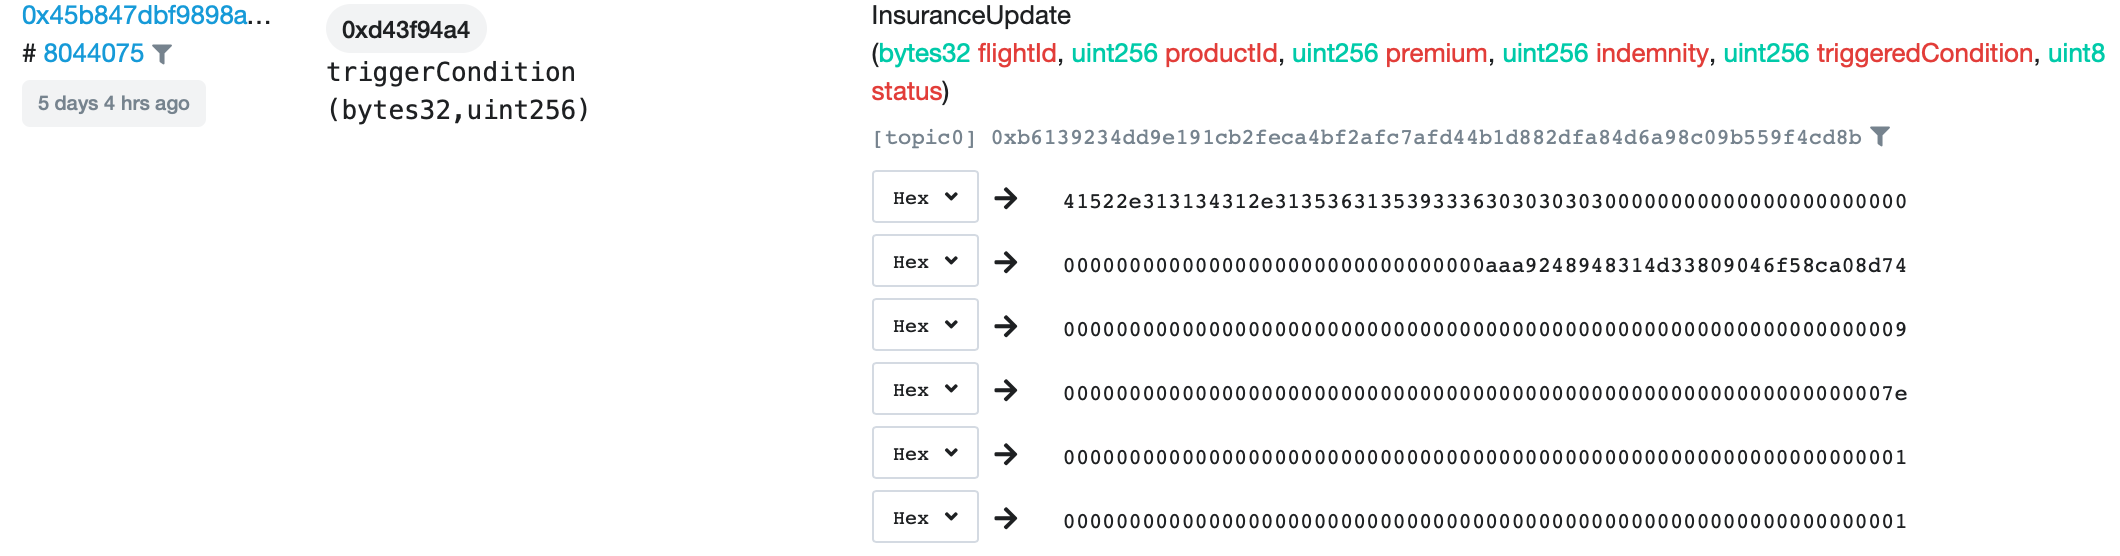
\includegraphics[width=\textwidth]{Bilder/FizzyExampleTrigger.png}
  \caption[Triggern einer Bedingung]{Triggern einer Bedingung \cite{FizzyTrigger2019}}
  \label{fig:fizzyTrigger}
\end{figure}

Fizzy ist nur eines von vielen Beispielen der Versicherungsbranche, die auf die Blockchain setzen. Es scheint so, als wäre auch hier ähnlich den Anfangsbestrebungen des B3i eher die Machbarkeit überprüft worden, anstatt alle gewohnten Prozesse auf Blockchain-Anwendungen und Smart Contracts umzustellen. Das belegen auch die Zahlen: Der alte Smart Contract umfasst ca. 20 000 Transaktionen \cite{EtherscanOldContract2019}, der neue noch nicht einmal eine dreistellige Anzahl \cite{EtherscanNewContract2019}. Dabei gilt zu berücksichtigen, dass 20 000 Einträge nicht 20 000 Versicherungen bedeutet, da mit dem Anlegen einer Versicherung und der Landung des Flugs mindestens zwei Methoden des darunterliegenden Contracts aufgerufen werden müssen. Dennoch ist die Umsetzung gelungen, da die Transparenz im Bezug auf die Bedeutung der einzelnen Parameter der Contract-Funktionen sehr positiv auffällt. So kann jeder die Abwicklung seines Fluges beobachten, ohne das persönliche Daten offengelegt werden. Trotzdem stellt sich auch hier wieder die Frage, inwiefern der Einsatz einer Blockchain-Lösung Vorteile bringt. Die Abwicklung der Kompensation kann zwar durch die eingebauten Trigger automatisch von Statten gehen, dennoch wird ein System für das Anlegen der Versicherung inklusive Datenhaltung für persönliche Daten und Zahlungsdaten benötigt. Hinzu kommen noch die Transaktionsgebühren der Ethereum Blockchain.




\chapter{Energieversorgung}
\label{chap:Energieversorgung}
\chapter{Hilfsgelder}
\label{chap:Hilfsgelder}
Zum Abschluss der Beispiele soll eine Anwendung von Smart Contracts aufgezeigt werden, die sich grundlegend von den anderen bereits vorgestellten unterscheidet. Wurde bisher immer von einem Business-Use-Case ausgegangen, können auch komplett unterschiedliche Felder von Smart Contracts profitieren. So auch die Verteilung von Hilfsgeldern, wie sie unter anderem von der UN gepflegt wird. 

Ein 
\chapter{Fazit und Ausblick}
\label{chap:FazitUndAusblick}
Blockchain und Smart Contracts sind zweifelsohne eine sehr spannende Thematik. Die Bewertung, ob sie allerdings die \enquote{Jahrhundertechnologie} ist, wird offen gelassen und anderen Personen überlassen. Ähnlich wurde in den 80er- und 90er-Jahren des letzten Jahrtausends die Objektorientierung als das Wunderwerk und die Lösung für alle Probleme gesehen. Das erinnert sehr an das Prinzip \emph{Golden Hammer}, wie es der US-amerikanische Psychologe Abraham Maslow in den 60-Jahren beschrieben hat: Ein Lösungsweg der scheinbar überall anwendbar ist. Ob Blockchain und Smart Contracts also den Hype überstehen, lässt sich sowieso erst im Rückblick beurteilen.

Wie an den Beispielen klar wurde, gibt es viele Bereiche im Business to Business und Business to Consumer Bereich, in denen Smart Contract eingesetzt werden können. Manches, wie beispielsweise Tradelens, wurde bereits mit großen Skalierungsfaktoren etabliert. Bei diesem Beispiel ist allerdings in der Art der Umsetzung als geschlossenes System mit der eigentlichen Blockchain-Idee, wie sie Satoshi Nakamoto beschreibt, keine große Überschneidungsmenge mehr zu finden.

Schlussendlich ist die Technologie nur eine zu betrachtende Komponente der Gleichung. An anderer Stelle steht die rechtliche Grundlage von Smart Contracts wie sie Stand heute implementiert sind. Um der Rechtssprechung verschiedener Länder zu entsprechen, müssen die Contracts jeweils angepasst werden. Das heißt im Umkehrschluss, dass hier neben Programmierern auch Juristen bei der Implementierung herangezogen werden sollten. Darüber hinaus darf auch der Datenschutz nicht ins Hintertreffen geraten, da in der Blockchain abgespeicherte Daten unwiderruflich dort gespeichert sind. Bei einer neuen Rechtslage könnten so gewisse Forderungen aufgrund der Architektur nicht umgesetzt werden. Generell sind Regierungen bei der Bearbeitungen informationstechnischer Themen träge, was sich mit der Schnelllebigkeit einer globalisierten Internetstruktur kaum verhindern lässt. Dennoch fordern neue Themen schnelle Bearbeitung, um in immer mehr Fällen Rechtssicherheit herstellen zu können.

Spielen mehrere dieser Faktoren zusammen, könnten Smart Contracts ein neues Zeitalter im Bezug auf Verträge einläuten und ein Paradebeispiel für die Digitalisierung darstellen. Vergleichbar war es z.B. mit der Programmiersprache Java in den 90er-Jahren für die Objektorientierung, welche auch heute noch von großer Relevanz ist.


\pagenumbering{Roman}
%Literaturverzeichnis
\printbibliography
\appendix
%Abbildungen, die nicht im Text auftreten
%\chapter{Abbildungen}
\begin{figure}[H]
  \centering
  \includegraphics[width=\textwidth]{Bilder/Lieferantenauftrag.PNG}
  \caption{Anlegen eines neuen Lieferantenauftrages}
  \label{fig:liefAuftrag}
\end{figure}
\begin{figure}[H]
  \centering
  \includegraphics[width=\textwidth]{Bilder/Lieferantenauftrag_Produktdetail.PNG}
  \caption{Detailansicht eines Artikels eines Lieferantenauftrags}
  \label{fig:auftrDetail}
\end{figure}
\begin{figure}[H]
  \centering
  \includegraphics[width=\textwidth]{Bilder/Milch_Link.PNG}
  \caption{Verlinkung des Artikels Milch}
  \label{fig:verlArtikel}
\end{figure}
\begin{figure}[H]
  \centering
  \includegraphics[width=\textwidth]{Bilder/Uebersicht_Lieferantenauftrag.PNG}
  \caption{Übersicht Lieferantenauftrag}
  \label{fig:auftrUebersicht}
\end{figure}
\begin{figure}[H]
  \centering
  \includegraphics[width=\textwidth]{Bilder/Kaufbeleg.PNG}
  \caption{Kaufbeleg}
  \label{fig:kaufbeleg}
\end{figure}
\begin{figure}[H]
  \centering
  \includegraphics[width=\textwidth]{Bilder/Mitteilung_Qualitaetspruefung.PNG}
  \caption{Mitteilung für eine erforderliche Qualitätsprüfung}
  \label{fig:mittQual}
\end{figure}
\begin{figure}[H]
  \centering
  \includegraphics[width=\textwidth]{Bilder/Qualitaetskontrolle_auswaehlen.PNG}
  \caption{Auswahlmöglichkeiten bei der Qualitätsprüfung}
  \label{fig:auswQual}
\end{figure}
\begin{figure}[H]
  \centering
  \includegraphics[width=\textwidth]{Bilder/Qualitaetspruefung.PNG}
  \caption{Übersicht der Qualitätsprüfung}
  \label{fig:qualPruef}
\end{figure}
\begin{figure}[H]
  \centering
  \includegraphics[width=\textwidth]{Bilder/Zahlung.PNG}
  \caption{Zahlung mit Rechnungsverknüpfung}
  \label{fig:zahlung}
\end{figure}
\begin{figure}[H]
  \centering
  \includegraphics[width=\textwidth]{Bilder/Auftrag_Mail.PNG}
  \caption{Lieferantenauftrag als PDF}
  \label{fig:auftrPdf}
\end{figure}
\begin{figure}[H]
  \centering
  \includegraphics[width=\textwidth]{Bilder/Arbeitsplatz.PNG}
  \caption{Arbeitsplatz \glqq Kessel\grqq}
  \label{fig:arbPlatz}
\end{figure}
\begin{figure}[H]
  \centering
  \includegraphics[width=\textwidth]{Bilder/Arbeitsgang.PNG}
  \caption{Arbeitsgang \glqq Lab hinzufügen\grqq}
  \label{fig:arbGang}
\end{figure}
\begin{figure}[H]
  \centering
  \includegraphics[width=\textwidth]{Bilder/Stueckliste.PNG}
  \caption{Stückliste für Gouda}
  \label{fig:stListe}
\end{figure}
\begin{figure}[H]
  \centering
  \includegraphics[width=\textwidth]{Bilder/Fertigungsauftrag.PNG}
  \caption{Fertigungsauftrag für Gouda}
  \label{fig:fertAuftr}
\end{figure}
\begin{figure}[H]
  \centering
  \includegraphics[width=\textwidth]{Bilder/Fertigungsauftrag_nicht_begonnen.PNG}
  \caption{Fertigungsauftrag (Herstellung noch nicht begonnen)}
  \label{fig:fertNichtBeg}
\end{figure}
\begin{figure}[H]
  \centering
  \includegraphics[width=\textwidth]{Bilder/Materialtransfer.PNG}
  \caption{Materialtransfer für die Herstellung}
  \label{fig:matTransfer}
\end{figure}
\begin{figure}[H]
  \centering
  \includegraphics[width=\textwidth]{Bilder/Lagerbuchung.PNG}
  \caption{Lagerbuchung für die Herstellung}
  \label{fig:lagBuchung}
\end{figure}


 
%\chapter{Anmerkungen}
Die enthaltenen Bilder sind allesamt Screenshots aus dem \gls{erp}-System oder wurden selbst erstellt (wie beispielsweise Abbildung \ref{fig:geschVorfall}).

Die gesamte Arbeit wurde mit einer von mir veränderten \LaTeX-Vorlage erstellt\footnote{Erreichbar unter: \url{https://github.com/latextemplates/scientific-thesis-template}.}. Diese ist zwar unter der freizügigen CC0 (= Public Domain) Lizenz veröffentlicht worden, verdient aber trotzdem (oder gerade deswegen) eine Würdigung.

Für die Coverpage wurde eine von mir veränderte Vorlage der Universität von Uppsala unter der CC BY 4.0 Lizenz verwendet\footnote{Erreichbar unter: \url{https://www.overleaf.com/latex/templates/uppsala-university-template/jvjprsfnzgbj#.Wzpz3dIzYuV}.}.
% Selbständigkeitserklärung
\chapter{Eidesstattliche Erklärung}
Hiermit erkläre und versichere ich, Lukas Willburger, Matrikel-Nr.\ 322445, dass ich die vorgelegte Studienarbeit mit dem Thema
\begin{quote}
\centering \textit{Anwendungen von Smart Contracts}
\end{quote}
selbständig verfasst und keine anderen als die angegebenen Quellen und Hilfsmittel benutzt habe, wobei ich alle wörtlichen und sinngemäßen Zitate als solche gekennzeichnet habe.  Dies gilt auch für Zeichnungen, Skizzen, bildliche Darstellungen sowie für Quellen aus dem Internet.
\\[6ex]

Dietmannsried, den \today \\


\rule[-0.2cm]{5cm}{0.5pt}

Lukas \textsc{Willburger} 
 

%\renewcommand{\appendixtocname}{Anhang}
%\renewcommand{\appendixname}{Anhang}
%\renewcommand{\appendixpagename}{Anhang}
%\input{latexhints-german}
%\input{latexhints-minted-german}

\pagestyle{empty}
\renewcommand*{\chapterpagestyle}{empty}
\end{document}
